%!TEX root = ../thesis.tex
%*******************************************************************************
%*********************************** Analysis Preservation *********
%*******************************************************************************

\chapter{Preservation and reusability}\label{ch:preservation}

\ifpdf
    \graphicspath{{chapter-preservation/Figs/Raster/}{chapter-preservation/Figs/PDF/}{chapter-preservation/Figs/}}
\else
    \graphicspath{{chapter-preservation/Figs/Vector/}{chapter-preservation/Figs/}}
\fi

Today's particle physics experiments are designed to collect physics data over a span over several decades. They thus operate at scales that makes it impossible for the experiments to be repeated in the foreseeable future. The data taken at these experiments and physics results derived are thus extremely valuable and major problems arise from a scientific reproducibility point of view. In this chapter, the reusability problems directly connected to an individual analysis are discussed, and approaches taken in view of analysis preservation and analysis reinterpretation are presented.

\section{The case for reinterpretations}\label{sec:reinterpretations}

\subsection{Motivation}
Designing and executing searches for \gls{bsm} physics requires a substantial amount of person-power and computing resources. As laid out in detail in \cref{part:simplified_model_analysis} of this thesis, an analysis generally aims to search regions in which a given \gls{bsm} model can be efficiently discriminated against \gls{sm} background. Although the careful design of such regions already requires significant amount of resources, it constitutes only a fraction of the work necessary for concluding the search. 
Contributions in the search regions from \gls{sm} processes need to be estimated, usually requiring expensive \gls{mc} simulation and the development of background estimation strategies. Systematic uncertainties arising from numerous sources need to be considered and estimated. 
For the \gls{bsm} signal, a similar processing pipeline involving \gls{mc} simulation, event reconstruction and event selection needs to be executed. Finally, recorded data also needs to be reconstructed and processed through the event selection. As shown in \cref{fig:pipeline_analysis}, an analysis can thus be divided into three main processing pipelines; a \textit{background pipeline}, \textit{signal pipeline} and \textit{data pipeline}. Only after all three processing pipelines are concluded can the next analysis step be performed---the \textit{statistical inference}, producing the final analysis results, like \eg limits on model parameters.

Due to the substantial amount of resources necessary for developing and performing an analysis, it is not feasible to develop dedicated searches for every possible \gls{bsm} scenario. Instead, analyses are typically only interpreted in a finite set of \gls{bsm} models that only have a small number of free parameters that need to be varied. Still, it is very likely that a given analysis is sensitive to a variety of different \gls{bsm} scenarios not considered in the original publication. 

Consequently, it is not surprising that there is significant interest in the \gls{hep} community to reinterpret \gls{bsm} searches in different signal models. Reinterpretations of published ATLAS searches for \gls{susy} are performed both within as well as outside of the ATLAS collaboration\improvement{some examples}. For the \gls{hep} community outside of the experimental collaborations, the results published by the analyses performed by the collaborations represent the only available windows into the dataset recorded, in the context of \gls{bsm} scenarios like \gls{susy}. Reinterpretations of reproducible analyses are thus the only possibility to determine the implications of \gls{lhc} data for a variety of models~\cite{reinterpretation_workshop}. Likewise, within the experimental collaborations, reinterpretations can additionally serve as a powerful tool for shaping the search program. Reinterpretations of ATLAS \gls{susy} searches in more complete \gls{susy} models like the \gls{pmssm} not only allow to state a combined sensitivity of ATLAS to more realistic \gls{susy} models, but also enable the collaboration to identify potential blind spots and parameter regions still uncovered by existing analyses. Such reinterpretations have been done in the past~\cite{pMSSM-scan-run1:2015baa,Ambrogi:2017lov} for the Run~1 dataset. Similar efforts aiming to reinterpret the current ATLAS search for \gls{susy} in the \gls{pmssm} using the full Run~2 dataset are currently ongoing. 

 \begin{figure}
	\centering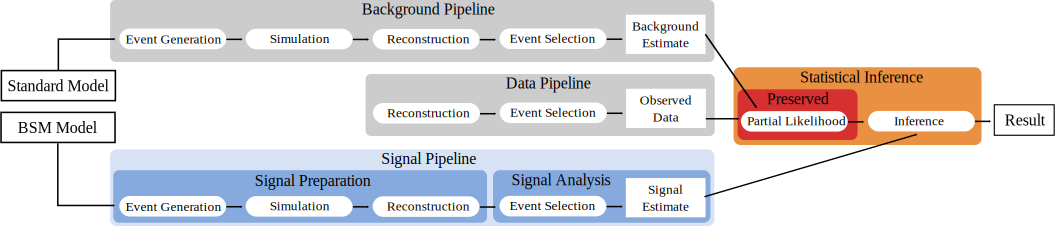
\includegraphics[width=\textwidth]{pipeline}
	\caption{Full analysis workflow including the three main processing pipelines for deriving background and signal estimates as well as observed data rates. The outputs of the three processing pipelines are combined into a likelihood forming the basis for statistical inference. In a \textsc{Recast} setup, the background and data paths are archived (\eg by preserving the partial likelihood created from the background estimates and the observed data), and the signal path is fully preserved such that it can be re-run at any time. Figure recreated from \reference\cite{ATL-PHYS-PUB-2019-032}.}
	\label{fig:pipeline_analysis}
\end{figure}

\subsection{Necessary ingredients}

As the event selection of an analysis is fixed, the background estimates and observed data in the targeted regions of interest do not change and can be archived in a suitable format. Reinterpreting a search in the light of a new signal model consequently only requires the signal pipeline in~\cref{fig:pipeline_analysis} to be run again, in order to derive the signal estimates that serve as input for the statistical inference. As the data and background processing pipelines shown in~\cref{fig:pipeline_analysis} only enter the statistical inference as estimated event rates, the volume of data that needs to be archived is significantly smaller than the original input data. As will be discussed in~\cref{sec:full_likelihood}, it has recently become technically possible to directly preserve the partial analysis likelihood built from the background estimates and observed data, including all details of the statistical model used for inference. Once the signal estimates are known, a new full analysis likelihood can be built, and the viability of the new signal model can be tested. 

Different approaches exist for deriving signal estimates for a new \gls{susy} scenario of interest. Manifestly the most precise approach involves running the original analysis software using a different \gls{bsm} model. As this requires to preserve the entirety of the original software environment including workflows used in the analysis, this is arguably the most involved approach. A framework designed to facilitate such an effort, called \textsc{Recast}, has originally been proposed in \reference\cite{RECAST_cranmer} and aims to provide the cyber-infrastructure necessary for such an effort. Through a web interface, physicists would provide an alternative \gls{bsm} model and request a reinterpretation of a search, which would trigger a computational workflow executing the original analysis and delivering the \textit{recasted} results. \Cref{sec:recast_implementation} discusses an attempt at fully preserving the \onelepton search presented in this thesis using the \textsc{Recast} paradigm. 

As the \textsc{Recast} implementations of ATLAS searches for \gls{susy} are, in practice, not publicly available in their entirety but only meant to be interacted with through a \textsc{Recast} request, the exact original implementation of the analysis selection is in general not readily available. For this reason, a number of public tools aiming to reimplement an approximated version of the event selections of various \gls{bsm} searches are available. Prominent examples include \textsc{CheckMate}~\cite{Checkmate2:2016npn,Checkmate:2013wra} and \textsc{MadAnalysis5}~\cite{MadAnalysis:2012fm}. ATLAS has internally maintained a similar catalogue of its \gls{susy} analyses and is publishing event selection snippets in C++ on \textsc{HEPData}~\cite{HEPData:2017ypu}. Recently, this package maintained by ATLAS, called \textsc{SimpleAnalysis}~\cite{simpleanalysis}, has been made publicly available, allowing the C++ snippets published to be run outside the collaboration.

As the full detector simulation requires access to the collaboration's detector description and is the most computationally expensive step in the signal pipeline, it is often approximated using simplified detector geometries and granularities, or even ignored altogether. 
The most commonly used package for fast detector simulation outside of the collaboration is \textsc{Delphes}~\cite{Delphes:2009tx}, which is used in \eg \textsc{CheckMate} and \textsc{MadAnalysis5}. Other packages like \eg \textsc{Rivet}~\cite{Rivet1:2010ar,Rivet2:2019stt} approximate the detector response using dedicated 4-vector smearing techniques, assuming that the detector response roughly factorises into the responses of single particles. Internally, ATLAS also uses a dedicated framework for 4-vector smearing techniques, used in scenarios where other fast simulation techniques are still too expensive. \Cref{sec:truth_smearing} discusses these dedicated smearing functions further.

Finally, instead of trying to estimate the signal rates of a new signal model using \gls{mc} simulation and (reimplemented) analysis event selections, some reinterpretation efforts like \eg \textsc{SModelS}~\cite{SModelS1:2013mwa,SModelS2:2017neo} use \textit{efficiency maps} encoding the selection efficiency of the analysis as a function of some of the analysis observables (typically the sparticle masses). Such efficiency maps are routinely published by the ATLAS \gls{susy} searches on \textsc{HEPData}, and allows for efficient reinterpretations as long as the signal efficiencies mostly depend on the signal kinematics and are largely independent from the specific details of the signal model~\cite{SModelS1:2013mwa}. For the analysis presented in the previous part of this work, the efficiency maps and further analysis data products are available at \reference\cite{HEPdata_1Lbb}. 

\section{Public full likelihood}\label{sec:full_likelihood}

The likelihood is arguably one of the most information-dense and thus valuable data products of an analysis. Without precise knowledge of the exact likelihood of the original analysis, approximations need to be made for the statistical inference \eg in terms of correlations between event rate estimates as well as the treatment of uncertainties. Recently, ATLAS has started to publish full analysis likelihoods built using the \textsc{HistFactory} \gls{pdf} template introduced in~\cref{ch:statistics}~\cite{ATL-PHYS-PUB-2019-029}. This extraordinary step towards more open and reproducible science has been praised by the theory community~\cite{REINP:2020pec} as it allows for considerably more trustful reinterpretations. This effort has been facilitated by the development of \texttt{pyhf} in conjunction with the introduction of a \texttt{JSON} specification fully describing the \textsc{HistFactory} template. As a pure-text format, the \texttt{JSON} likelihoods are human- and machine-readable, highly compressible and can easily be put under version control, all of which are properties that make them ideal for long-term preservation. 

The full likelihood (in \texttt{JSON} format) of the search for electroweakinos presented in the previous part of this work has been published~\cite{fullLH_1Lbb} and is not only heavily used in the following chapters, but also in various analysis reinterpretation and combination efforts currently ongoing in ATLAS. Several efforts outside of the ATLAS collaboration have already included the analysis likelihood into their reinterpretations, \eg \textsc{SModelS}~\cite{SModelS_pyhf:2020grj} and \textsc{MadAnalysis}~\cite{Goodsell:2020ddr,Fuks:2021wpe} both reporting significant precision improvements through the use of the full likelihood (as opposed to approximating the statistical model). Furthermore, the full likelihood of the search presented herein has recently been used to demonstrate the concept of scalable distributed statistical inference on \glspl{hpc}~\cite{Feickert:2021sua}. Through the \texttt{funcX} package~\cite{chard20funcx}, \texttt{pyhf} is used as a highly scalable \textit{function as a service} to fit the entire signal grid of 125 signal points with a wall time of $\SI{156}{\second}$ using 85 available worker nodes\footnote{Theses benchmarks use \texttt{pyhf}'s \textsc{NumPy} backend and \textsc{SciPy} optimiser, which does have a slower log-likelihood minimisation time than \eg \textsc{PyTorch} coupled with \textsc{SciPy}, as will be shown in \cref{sec:cpu_performance}.}.

\section{Full analysis preservation using containerised workflows}\label{sec:recast_implementation}

For an analysis to be fully re-usable under the \textsc{Recast} paradigm, the signal pipeline of the original analysis (see \cref{fig:pipeline_analysis}) needs to be preserved such that it can be re-executed on new inputs. As typically only the processing steps after the event reconstruction are analysis-specific, it is sufficient to preserve this part of the signal pipeline. Processing steps preceding the calibration and selection of physics objects only involve the central ATLAS production system and result in \textit{derived analysis object data} formats that are used by analyses. These processing steps are preserved using centrally provided infrastructure.

   In the following, the term \textit{analysis pipeline} will refer to the analysis-specific data processing steps that are not handled by the central ATLAS production system, typically starting with selection of events in the \textit{derived analysis object data} format\improvement{cite} that have passed the reconstruction step in~\cref{fig:pipeline_analysis}. Preserving the analysis pipeline not only needs preservation of the full software environment for the different data processing steps, but also knowledge about the correct usage of the software through parameterised job templates together with a workflow graph connecting the different steps.

\subsection{Software preservation}

As much of the software is only tested, validated and deployed on a narrow set of architectures and platforms, the full software environment defining an analysis pipeline not only includes the original analysis-specific code used for object definitions, calibrations, event selection and statistical inference, but also the operating system used and a number of low-level system libraries that the applications depend upon. This can be achieved through the use of \textit{Docker containers}~\cite{docker,Binet:2134524} that---except for the operating system kernel---are able to package the full software environment, including a layered file system, the operating system as well as the actual application and all of its dependencies in a portable data format. As opposed to full virtualisation, Docker containers do not rely on hardware virtualisation but share the operating system kernel with host. Docker containers thus only interact with the host through system calls to the Linux kernel~\cite{ATL-PHYS-PUB-2019-032}\improvement{different source?} via a highly stable interface. This makes Docker containers a well-suited solution for deploying isolated applications on a heterogeneous infrastructure.

Due to the software structure of the analysis presented in this work, a containerisation requires a total of three container images spanning the following processing steps:
\begin{itemize}
	\item Event selection and physics object calibration: this step reads events in the \textit{derived analysis object data} format and produces flat \textsc{ROOT} files.
	\item Generation of expected signal rates: the histogram-building features of \textsc{HistFitter} are exploited to generate the necessary signal histograms in the relevant selections including all systematic variations. The histograms are subsequently converted into a \textsc{JSON} patch file that can be used to patch the partial likelihood.
	\item Statistical inference: although the original analysis used \textsc{HistFitter} for the statistical inference, the \textsc{Recast} implementation uses the \texttt{pyhf}-implementation of the \textsc{HistFactory} models in order to benefit from the possibility of using a partial \texttt{JSON} likelihood to preserve background and data rates. The \textsc{HistFitter} and \texttt{pyhf} implementations of the statistical inference have been shown to produce exactly the same results up to machine precision.
\end{itemize}

The first Docker image is based on a \textit{base image} providing a fixed ATLAS software release including all dependencies, expanded with the relevant analysis software. The second docker image uses the \textsc{ROOT} installation version originally used in the analysis, provided as part of a suitable ATLAS software release. The last image is based on a \texttt{pyhf} base image containing the \texttt{pyhf} release version used when validating the two \textsc{HistFactory} implementations against each other in the context of the analysis. All docker images are subject to version control and continuous integration, such that changes to the underlying software environment can be tracked and tagged. This allows for a consistent preservation of multiple versions of the analysis pipeline. \improvement{provide dockerfiles in appendix}

\subsection{Processing steps preservation}

Preserving the software environment is not sufficient, as detailed instructions on how to use it have to be given to the user. This is achieved through parameterised job templates that specify the precise commands and arguments required to re-execute the analysis code for specific processing steps. As re-executing the analysis pipeline using different signal models involves varying input parameters, all job template parameters are exposed to the user. Within \textsc{Recast}, the job templates are formulated using the YAML format. 

User-specifiable arguments and inputs to the event selection and physics object calibration step include the actual reconstructed \gls{mc} events in \textit{derived analysis object data} format, obtained through the central ATLAS production system, as well as corresponding files necessary for the pile-up correction in \gls{mc}. In addition, the signal process cross section as well as \gls{mc} generator-level efficiencies need to be given for correct normalisation the estimated signal rates to the integrated luminosity of the full Run~2 dataset. For each new signal model to be tested, three \gls{mc} samples need to be provided, generated with specific pile-up profiles close to the pile-up profile in data during the 2015--2016, 2017 and 2018 data-taking periods, respectively\footnote{This allows to have pile-up weights close to unity, avoiding unnecessary statistical dilution.}. In all three jobs, the events processed are weighted according to the integrated luminosity of the data-taking period they represent within the full Run~2 dataset. A subsequent \textit{merging} step uses the same docker image as the previous processing step, and serves to merge the three produced outputs into a single \textsc{ROOT} file that can be read by the subsequent step.

Apart from the merged \textsc{ROOT} output file produced in the previous step, the generation of the expected signal rates in a \texttt{JSON} patch format requires only one additional input---a \texttt{JSON} file containing theory uncertainties on the expected signal rates. These are optional and do not have to be specified if deemed to be negligible for the signal model to be tested.

The statistical inference steps requires the signal \texttt{JSON} patch from the previous step as well as the archived partial likelihood containing observed data as well as expected background rates including systematic variations thereof. 

\subsection{Workflow preservation}

Finally, the preserved processing steps need to be linked together, creating a parameterised workflow completely defining the analysis pipeline from centrally produced \gls{mc} datasets to the statistical inference results. Within \textsc{Recast}, this is achieved using the workflow description language \texttt{yadage}~\cite{yadage:2017frf}, capturing the full workflow in YAML format. The workflow uses the job templates and defines their processing order and dependencies. \Cref{fig:recast_workflow} shows a graph visualisation of the entire analysis pipeline, implemented in \textsc{Recast}. 

The \textsc{Recast} implementation of the analysis presented in this work has been validated against original analysis inputs. The expected and observed CL$_s$ values derived in the original analysis could be re-derived using the containerised workflow implementation. On a non-isolated CPU, the full preserved analysis pipeline for a single signal model can be executed within 1 hour. Due to the highly portable nature of the containerised workflow, the pipeline can easily be run in a distributed setup, allowing scalable reinterpretations at full analysis precision. 


 \begin{sidewaysfigure}[ht]
	\centering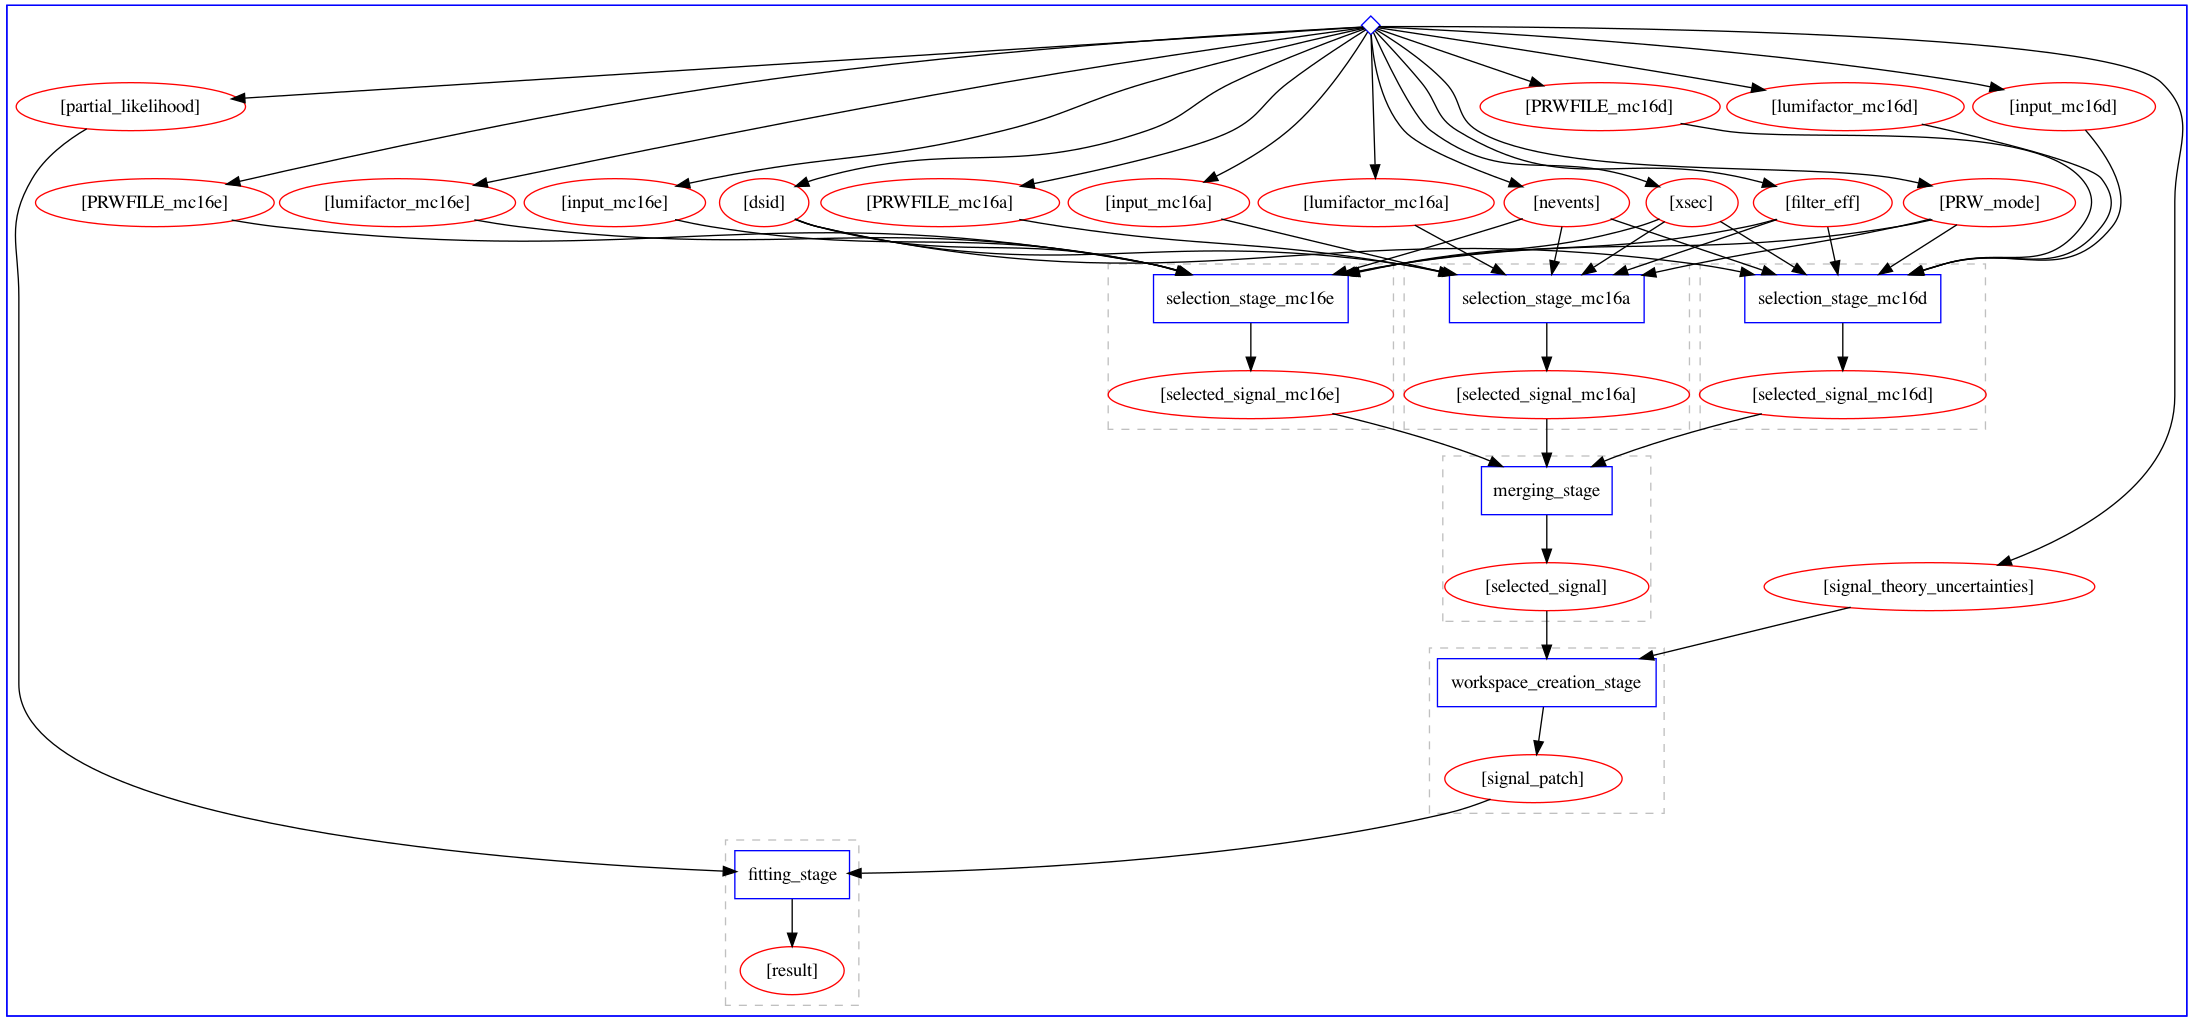
\includegraphics[width=\textwidth]{yadage_workflow_instance}
	\caption{Graph of the workflow as specified for the analysis pipeline. The containerised processing steps are represented as blue rectangular nodes, while input parameters, input files and outputs are shown as red oval nodes. The workflow is comprised of four processing steps: \texttt{selection\_stage\_mc16(a,d,e)}, \texttt{merging\_stage}, \texttt{workspace\_creation\_stage} and \texttt{fitting\_stage}. The first two steps perform the object calibration, event selection and merging of the three \gls{mc} datasets representing the three data-takin periods 2015--2016, 2017 and 2018. The latter two steps implement the generation of the signal \texttt{JSON} patch as well as the final statistical inference. Compared to \cref{fig:pipeline_analysis} the first two steps implement the \textit{signal analysis} part, while the latter two steps implement the \textit{statistical inference} deriving the final results.} 
	\label{fig:recast_workflow}
\end{sidewaysfigure}

\section{Simplified analysis preservation}\label{sec:simplified_preservation}

A full preservation of the entire analysis pipeline is highly desirable as it allows for a maximum precision reinterpretation of the original analysis in a new, promising signal model. As the full detector simulation needs a significant amount of CPU resources in addition to the non-negligible wall time of the actual preserved analysis pipeline, this approach can only be used on a limited set of models. In large-scale reinterpretations over high-dimensional parameter spaces, the amount of unique models that need to be sampled and investigated using the analysis is too high to employ the fully preserved analysis pipeline. In order to significantly reduce the wall time needed for passing through the analysis pipeline, a number of approximations and simplifications have to be made. 

In the following chapters, two major simplifications are discussed, targeting both the \textit{signal pipeline} as well as the \textit{statistical inference} blocks in~\cref{fig:pipeline_analysis}. \Cref{ch:simplify} introduces a procedure for building simplified likelihoods out of the published full likelihoods of ATLAS SUSY searches in order to significantly lower the wall time needed for running statistical fits in an analysis. \Cref{ch:pmssm} discusses an approach to approximate the \textit{signal pipeline} preceeding the statistical inference by resorting to truth-level analysis and approximating the detector response using dedicated smearing functions instead of running the full detector simulation. Both approximations are finally combined into a \textit{simplified analysis pipeline} and applied on a set of \gls{susy} models sampled from the \gls{pmssm}. 


\ifpdf
    \graphicspath{{chapter-pmssm/Figs/Raster/}{chapter-pmssm/Figs/PDF/}{chapter-pmssm/Figs/}}
\else
    \graphicspath{{chapter-pmssm/Figs/Vector/}{chapter-pmssm/Figs/}}
\fi


\section{Truth-level analysis}\label{sec:truth_analysis}

As discussed in~\cref{ch:preservation}, the reinterpretation of an analysis involves re-executing the analysis pipeline in order to derived signal rate estimates in all regions. In large-scale reinterpretations, running a \textsc{Recast} implementation on all signal models considered is not computationally feasible and instead a \textit{truth-level} analysis is first performed for all signal models sampled. Only models with uncertain exclusion at truth-level are processed through the computationally expensive full analysis chain implemented in \textsc{Recast}. The truth-level analysis skips the detector simulation and uses generator-level objects instead. Any detector-level effects and inefficiencies will thus not be reflected in truth-level observables. In order to reproduce the kinematic distributions observed in the full analysis (using reconstruction-level objects), a dedicated \textit{truth smearing}---discussed in detail in~\cref{sec:truth_smearing}---is applied.

\subsection{Truth selection}\label{sec:truth_selection}

 \begin{figure}
	\centering
	\begin{subfigure}[b]{0.45\linewidth}
		\centering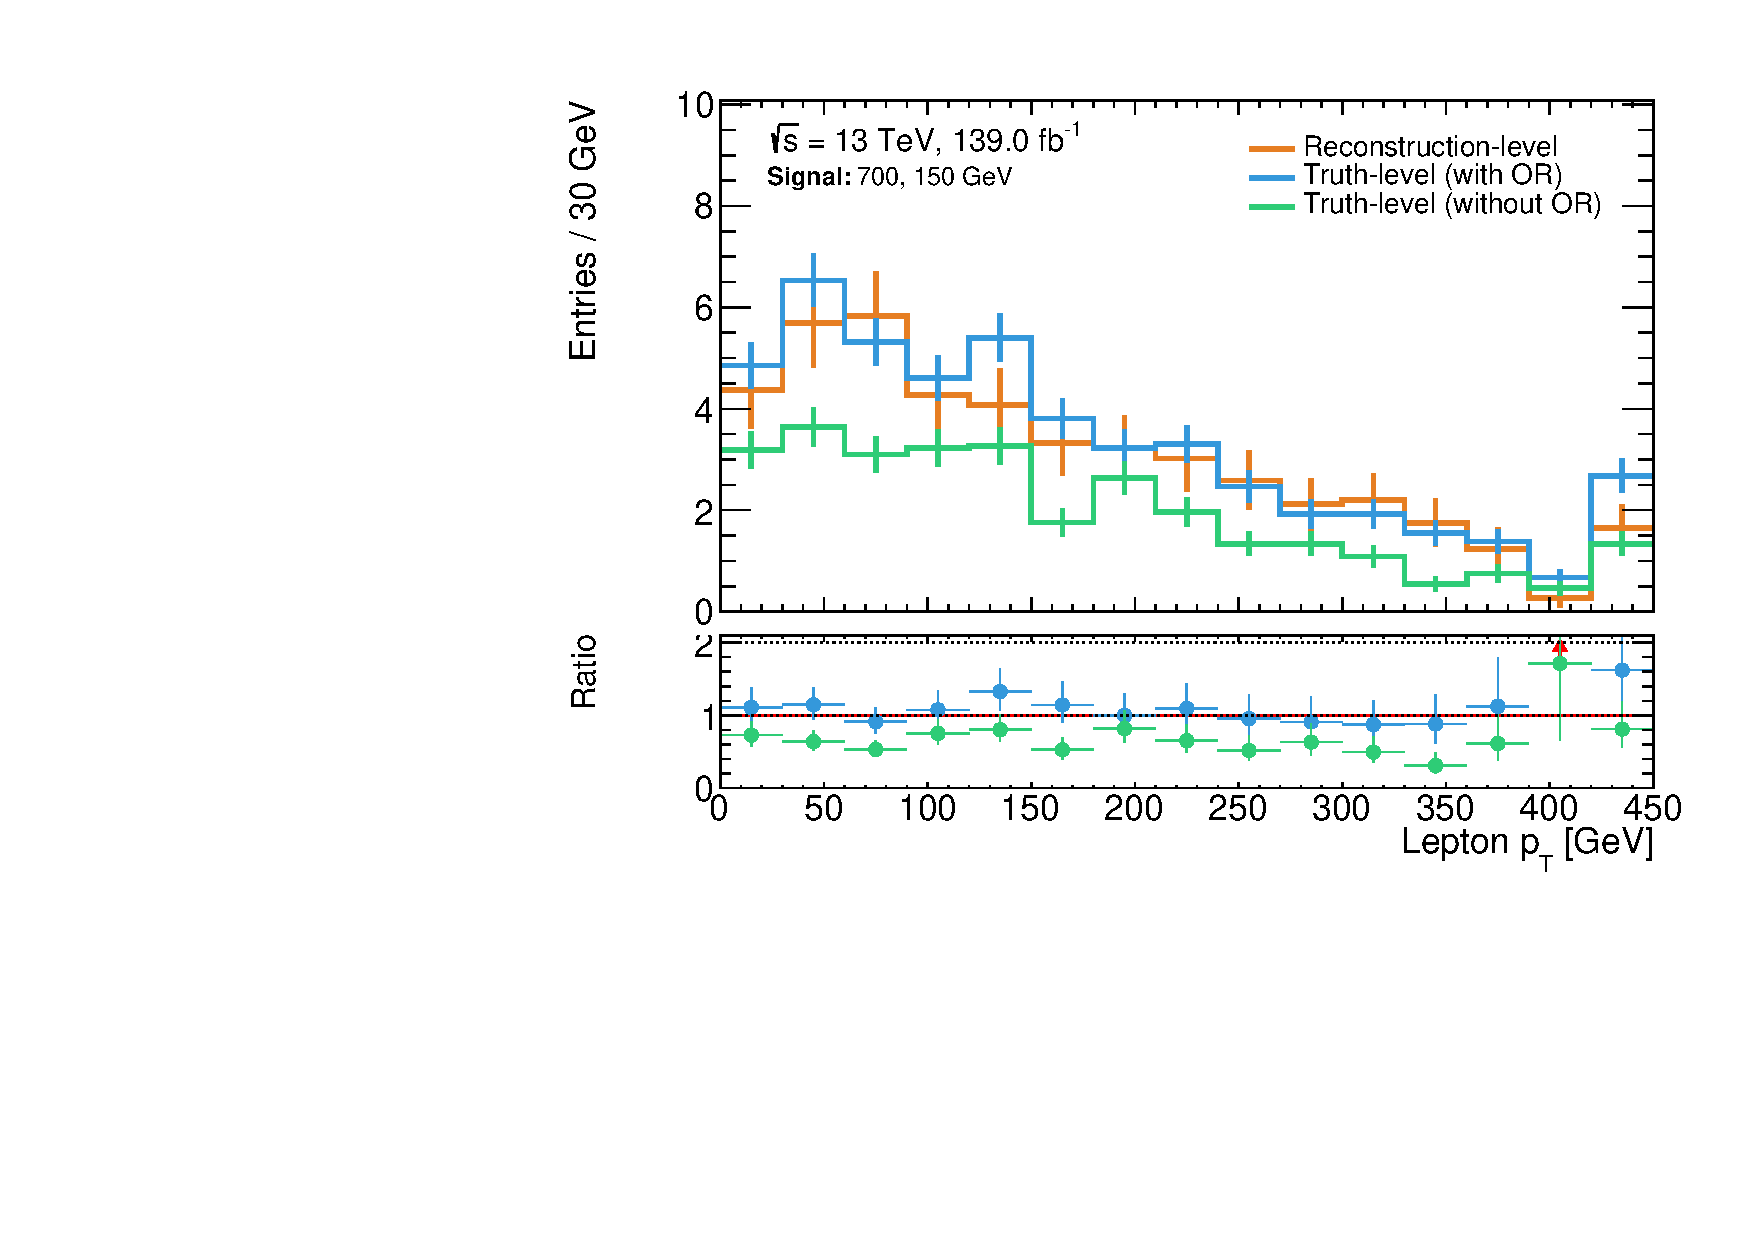
\includegraphics[width=\textwidth]{20210324_noLabel_noOR/700_150/lep1Pt_C1N2_Wh_hbb_700p0_150p0_smeared.pdf}
	\end{subfigure}\hfill
	\begin{subfigure}[b]{0.45\linewidth}
		\centering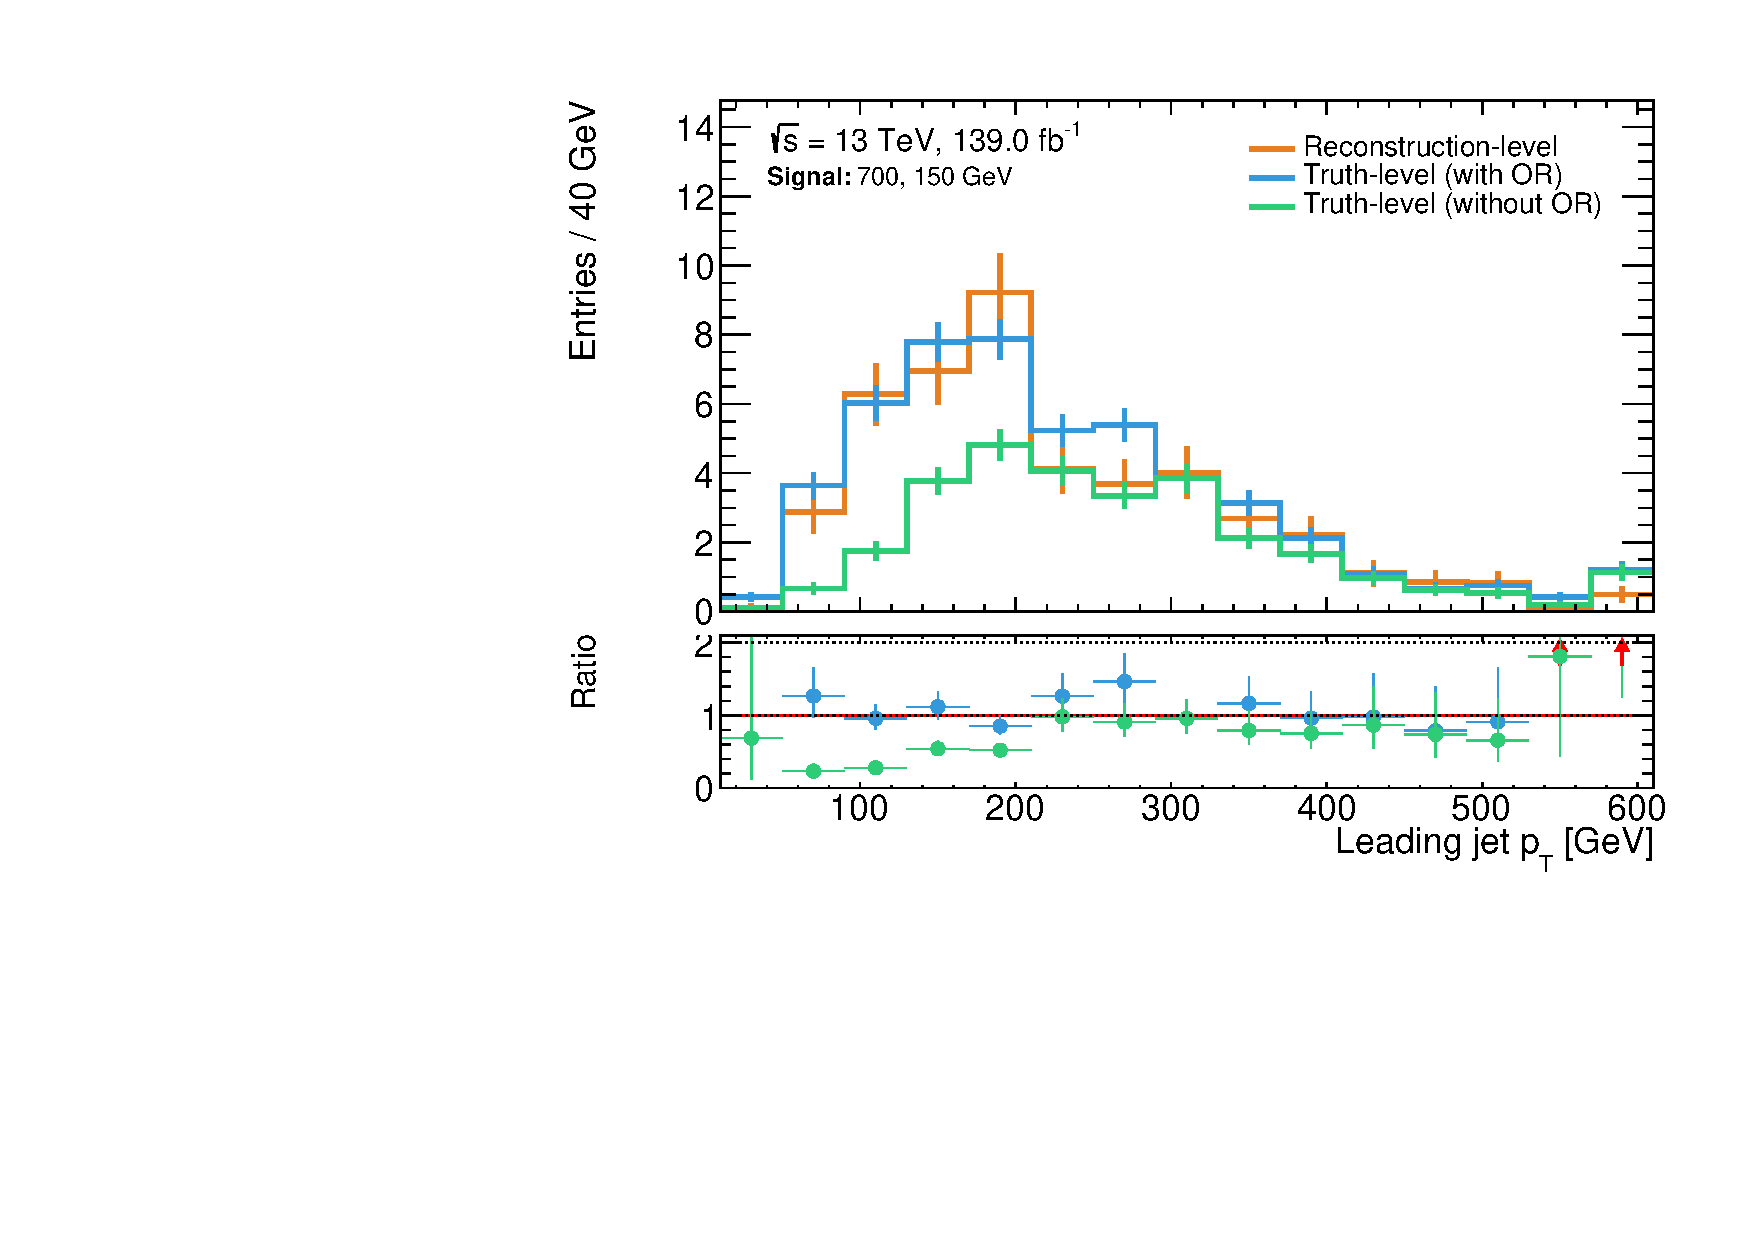
\includegraphics[width=\textwidth]{20210324_noLabel_noOR/700_150/jet1Pt_C1N2_Wh_hbb_700p0_150p0_smeared.pdf}
	\end{subfigure}\hfill
	\caption{Impact of the overlap removal procedure at truth-level illustrated in the lepton and leading jet transverse momenta distributions. The truth-distribution without overlap removal (green) generally underestimates the number of signal events at reconstruction-level (orange). Correct overlap removal procedure at truth-level (blue) improves the agreement. The exemplary benchmark signal point with $m(\charg/\neutr), m(\lsp) = 700, \SI{150}{\GeV}$ is shown in both plots (at truth- and reconstruction-level). All distributions are shown in a loose preselection requiring exactly one lepton, $\met>\SI{50}{\GeV}$, $\mt > \SI{50}{\GeV}$, and 2--3 jets, two of which need to be \textit{b}-tagged.}
	\label{fig:overlap_removal_truth}
\end{figure}

All signal and control regions considered in the original 1-lepton search are implemented at truth-level using \textsc{SimpleAnalysis}. The exact implementation is publicly available at \reference\cite{HEPdata_1Lbb} and was already used in~\cref{ch:uncertainties} for the derivation of some of the theory uncertainties in the full analysis.

The truth-level implementation full specifies all object definitions introduced in~\cref{sec:object_definitions} even though some of them, like \eg lepton isolation, are technically not well-defined at truth-level The subsequent smearing is in many cases implemented as a function of said object definitions and thus allows to consider them nonetheless. Additionally, as discussed in~\cref{sec:reinterpretations}, the full specification of the original analysis event selection including all object definitions allows for simpler reinterpretations by efforts outside of the ATLAS collaboration that generally do not have access to the original analysis software.

Following the object definitions, an overlap removal procedure following the same prescription as described for the reconstruction-level analysis is performed, \ie especially also using the same shrinking cone definitions introduced in~\cref{sec:overlap_removal}. Overlap removal step removing electrons sharing a track with a muon is approximated by using a distance parameter of $\Delta R = 0.01$ between the objects. Although often neglected\footnote{The overlap removal procedures in ATLAS \gls{susy} searches tend to be quite intricate, making them non-trivial to re-implement without ATLAS and analysis-specific knowledge.} in reinterpretation efforts outside of the collaboration, the correct implementation of the overlap removal procedure employed in the original analysis is typically crucial to reproduce the signal estimates of the original analysis, as illustrated in~\cref{fig:overlap_removal_truth}. Furthermore, the exact implementation of all analysis observables is explicitly given in the \textsc{SimpleAnalysis} implementation, followed by the full definition of all control and signal regions.

\subsection{Truth smearing}\label{sec:truth_smearing}

The general assumption of the truth smearing applied in the following is that the detector response roughly factorises into the responses of single particles. This allows to use detector performance results provided by ATLAS in order to construct detector response maps parameterised in different observables for each physics object. Detector response maps include object reconstruction and identification efficiencies as well as scale factors to correct for differences between \gls{mc} and observed data. Likewise, effects from the finite resolution of energy measurements in the detector are modelled through energy resolution maps. In the following, the 4-vector components of electrons, muons, jets and $\etmiss$ are smeared. The implementation of the smearing functions is internal to ATLAS and originates predominantly from various upgrade studies.

In the case of truth electrons, the identifications efficiencies considered are parameterised in $\eta$ and $\pt$ as well as the identification working point used. In $\eta$, nine fixed-width bins are used. In $\pt$, six bins are implemented and a linear interpolation between two adjacent $\pt$-bins is used to get the efficiency for the given $\pt$ of each truth electron. The probability of finding a fake electron in a truth jet is estimated through a similar two-dimensional map depending on the truth jet $\eta$ and $\pt$, again using fixed-width bins in $\eta$ and a linear interpolation in $\pt$. The range of the $\pt$ interpolation for identification efficiencies and fake rates extends from $\SI{7}{\GeV}$ to $\SI{120}{\GeV}$. If the truth $\pt$ of the electron is outside of that range, the identification efficiency and fake rate from the respective bound of the corresponding $\eta$-bin are used. The probability for misidentifying an electron as a photon is estimated using different fixed values for the barrel and end-cap regions. Finally, the transverse energy of the electron is smeared using a random number drawn from a Gaussian distribution with  standard deviation corresponding to the $\eta$- and $\pt$-dependent energy resolution.  

For truth muons, the identification efficiencies are also parameterised in $\eta$ and $\pt$ as well as the identification working point used. Similar to truth electrons, the  $\pt$ of the muon is smeared using a Gaussian distribution with standard deviation corresponding to the momentum resolution. The momentum resolution of combined truth muons, $\sigma_\mathrm{CB}$, is computed from the measured resolutions in the \gls{id},$\sigma_\mathrm{ID}$, and \gls{ms}, $\sigma_\mathrm{MS}$, as
\begin{equation}
	\sigma_\mathrm{CB} = \frac{\sigma_\mathrm{ID}\sigma_\mathrm{MS}}{\sqrt{\sigma_\mathrm{ID}^2 + \sigma_\mathrm{MS}^2}},
\end{equation}
where $\sigma_\mathrm{ID}$ and $\sigma_\mathrm{MS}$ are parameterised in $\eta$ and $\pt$.

The transverse momentum of truth jets is smeared using a Gaussian with standard deviation equal to the \gls{jer}, provided in a map parameterised in five bins in $\eta$ ranging from $\vert\eta\vert = 0$ to $\vert\eta\vert = 4.5$. Following~\cite{Aad:2020flx}, jet energy resolutions are provided using parameterisations of a noise $N$, stochastic $S$ and constant $C$ term for each of the seven bins in $\vert\eta\vert$, such that the resolution can be computed as
\begin{equation}
	\frac{\sigma(\pt)}{\pt} = \frac{N}{\pt}\oplus\frac{S}{\sqrt{\pt}}\oplus C.
\end{equation}
Only truth jets with $\SI{10}{\GeV} < \pt < \SI{1.5}{\TeV}$ are smeared. For truth jets with $\pt > \SI{20}{\GeV}$, the flavour tagging efficiency is considered using efficiencies parameterised in $\eta$, $\pt$ and the \textsc{MV2c10} working point (introduced in~\cref{sec:object_definitions}) used, measured in fully reconstructed simulated $\ttbar$ events~\cite{FTAG-2018-01}.

Finally, the smeared missing transverse energy is computed using the transverse momenta of all smeared truth objects in the event, including an approximation for the track soft term. The latter is approximated using results from $Z\rightarrow e^+e^-$ events, allowing to infer a distribution of the mean soft term projected in the direction longitudinal to the total transverse momentum of all hard objects in an event, $\boldsymbol{p}_\mathrm{T}^\mathrm{hard}$. The measured resolution parallel and perpendicular to $\boldsymbol{p}_\mathrm{T}^\mathrm{hard}$ is then used to smear the nominal soft track value.
 
  \begin{figure}
	\centering
	\begin{subfigure}[b]{0.45\linewidth}
		\centering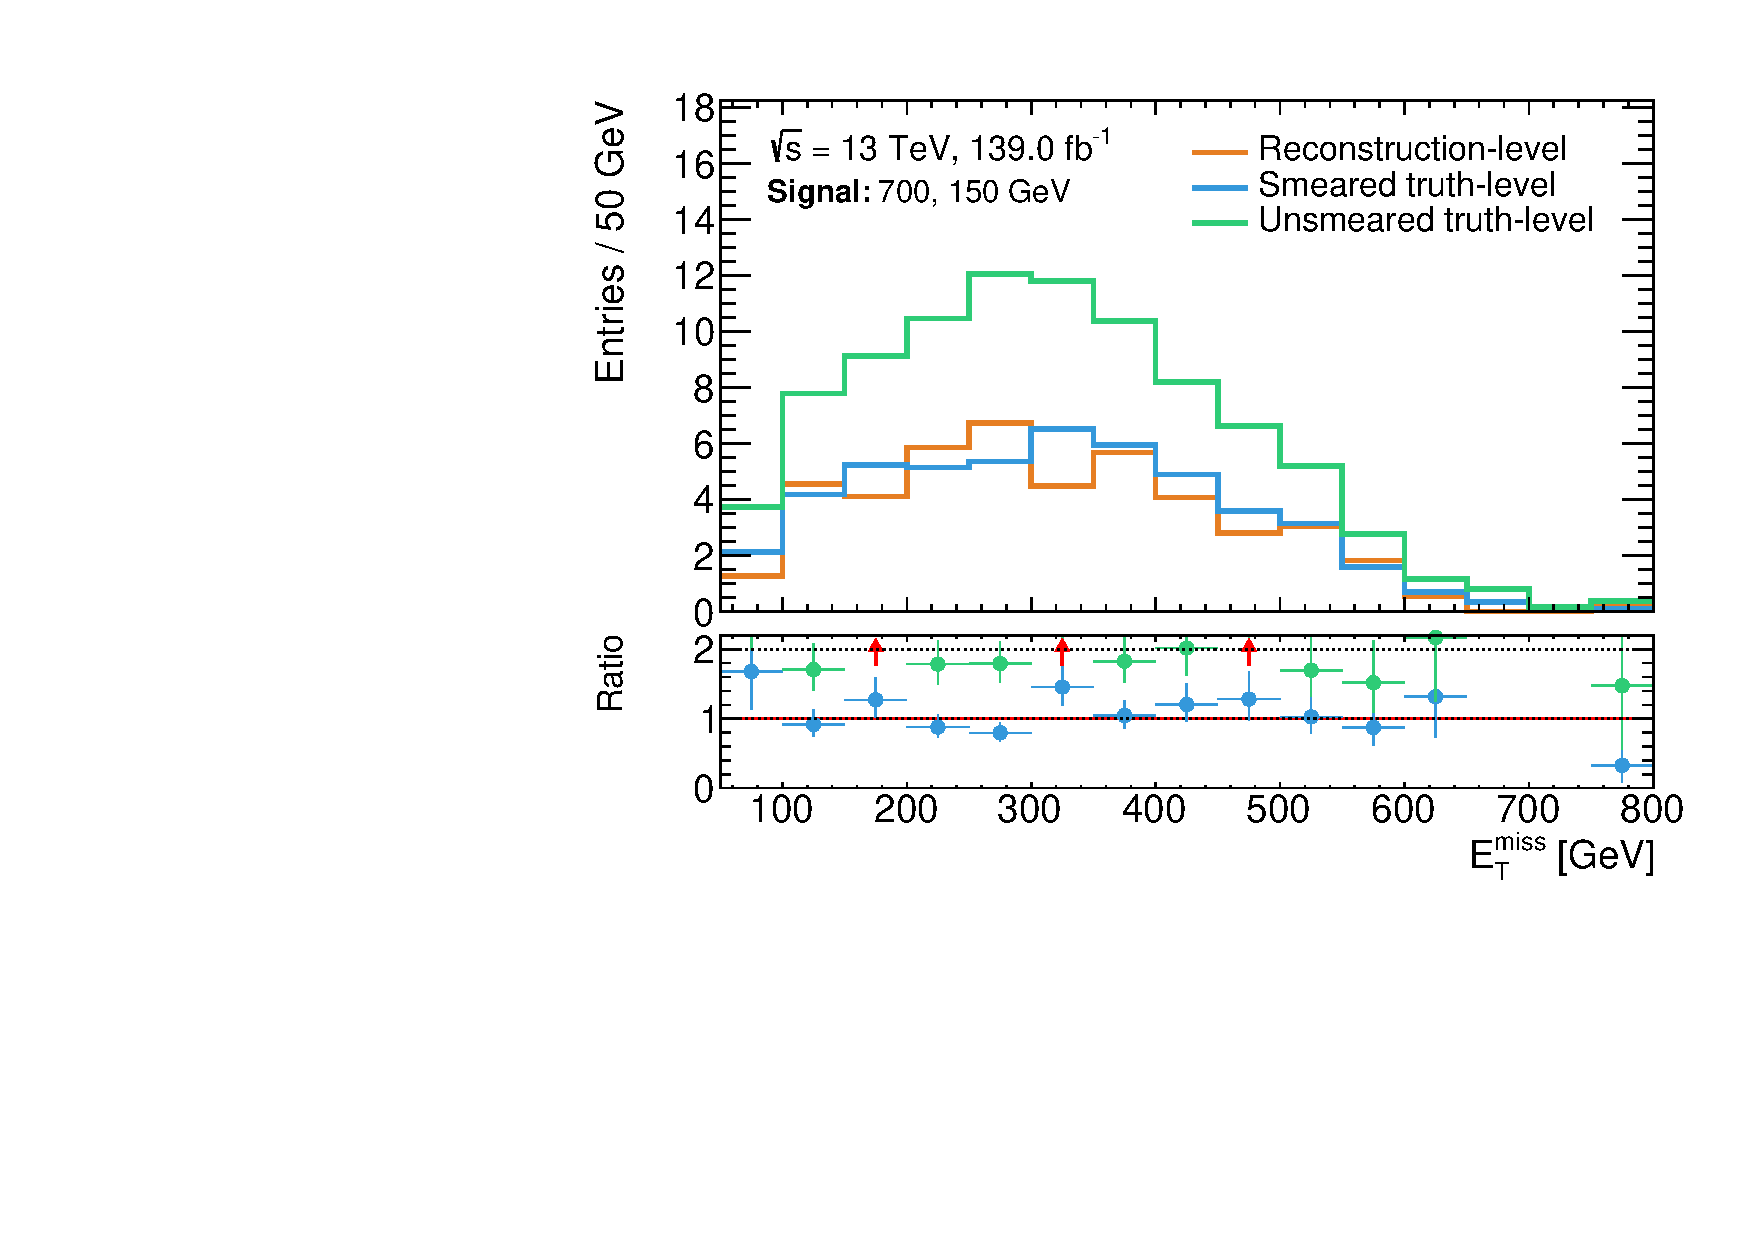
\includegraphics[width=\textwidth]{20210324/700_150/met_C1N2_Wh_hbb_700p0_150p0_smeared.pdf}
	\end{subfigure}\hfill
	\begin{subfigure}[b]{0.45\linewidth}
		\centering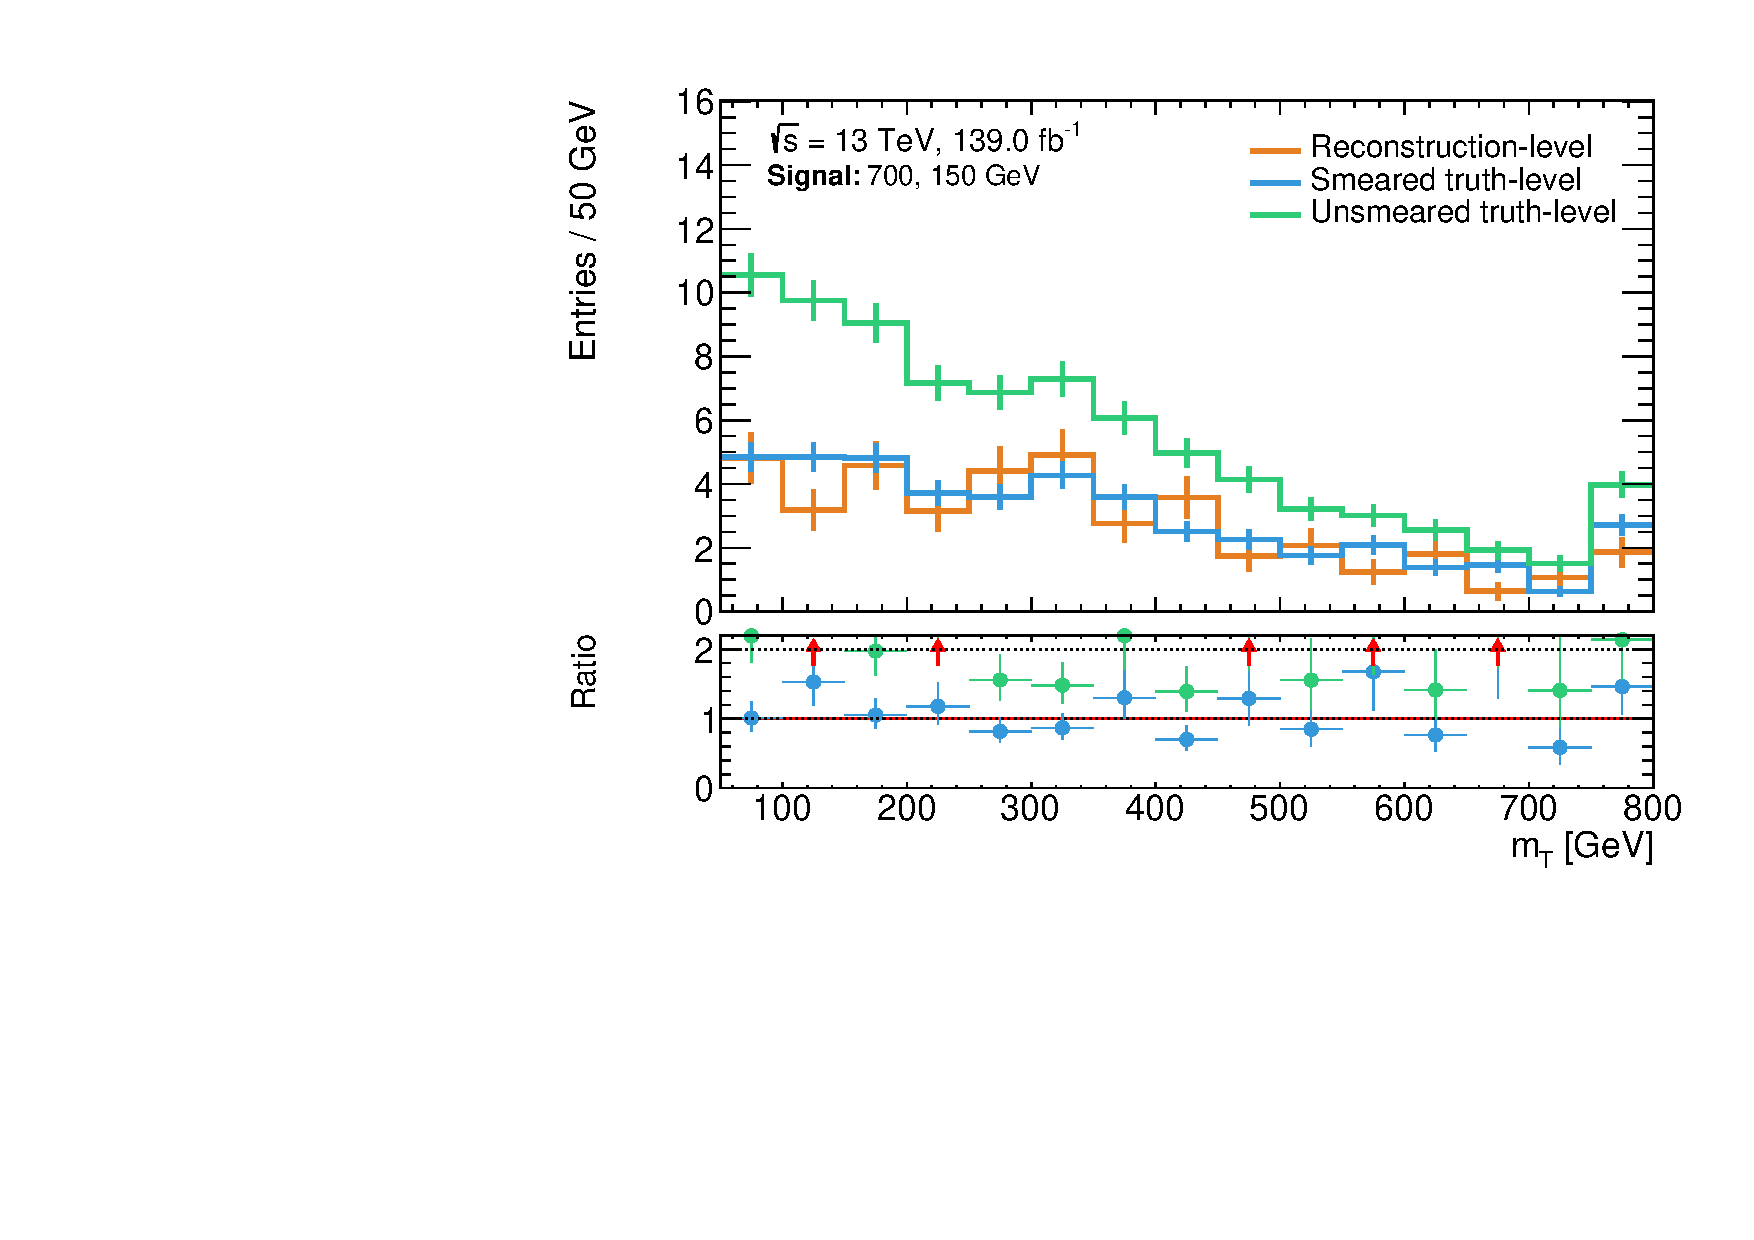
\includegraphics[width=\textwidth]{20210324/700_150/mt_C1N2_Wh_hbb_700p0_150p0_smeared.pdf}
	\end{subfigure}\hfill
	\begin{subfigure}[b]{0.45\linewidth}
		\centering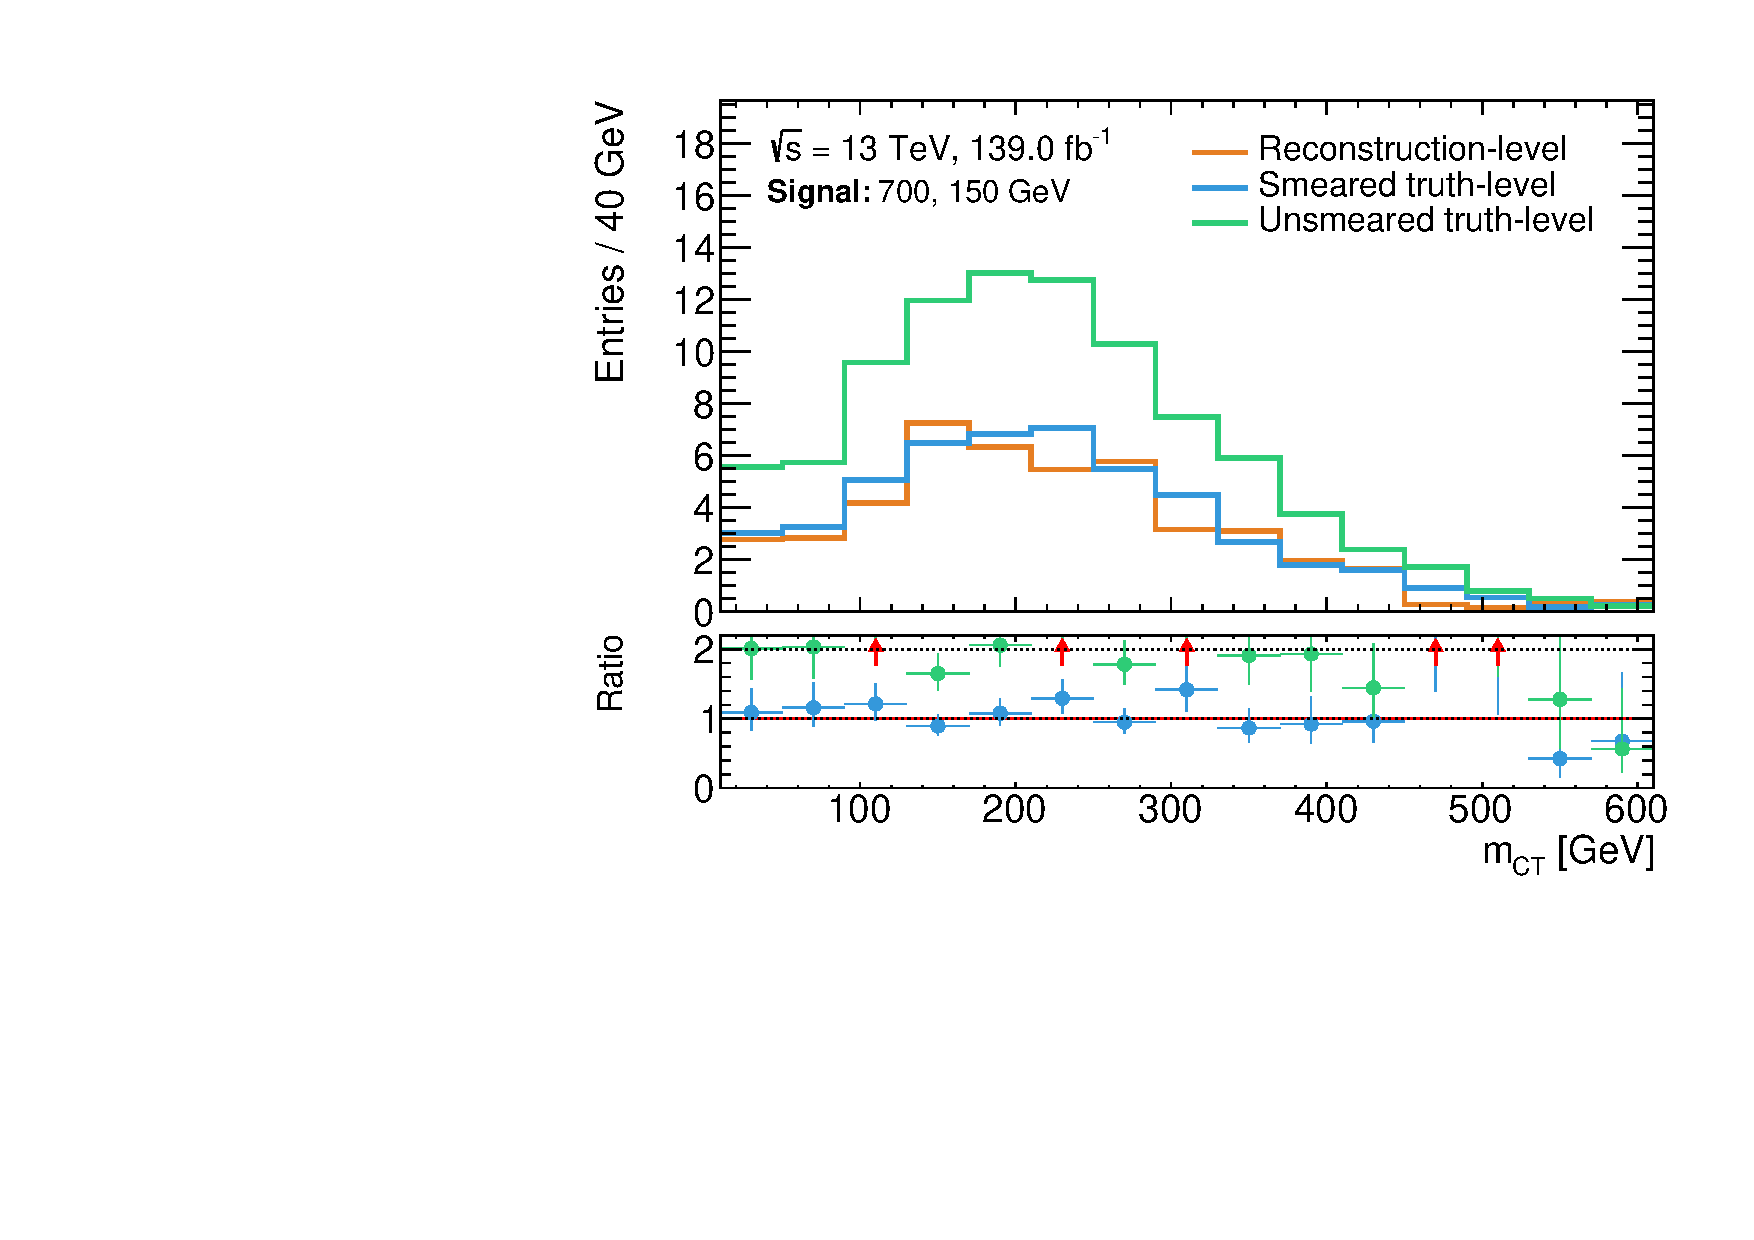
\includegraphics[width=\textwidth]{20210324/700_150/mct_C1N2_Wh_hbb_700p0_150p0_smeared.pdf}
	\end{subfigure}\hfill
	\begin{subfigure}[b]{0.45\linewidth}
		\centering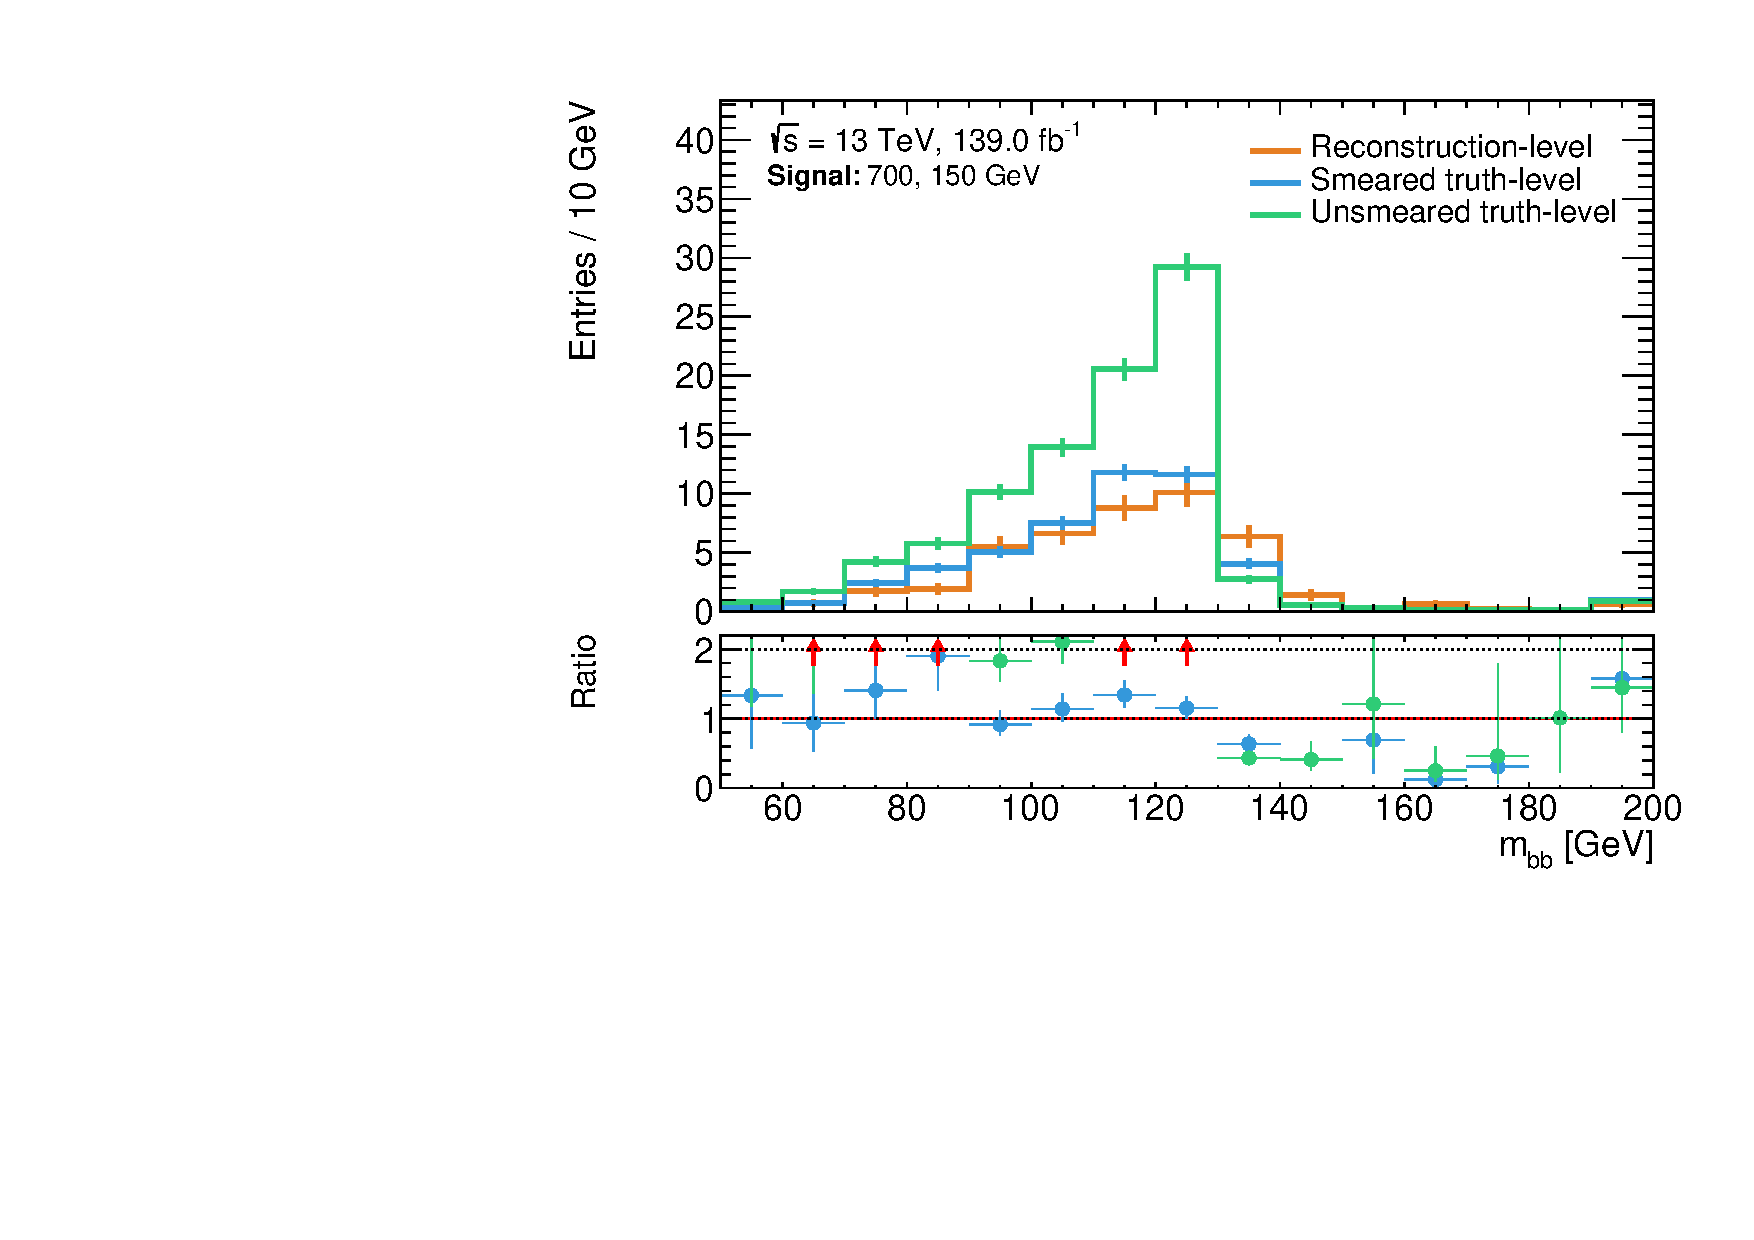
\includegraphics[width=\textwidth]{20210324/700_150/mbb_C1N2_Wh_hbb_700p0_150p0_smeared.pdf}
	\end{subfigure}\hfill
	\begin{subfigure}[b]{0.45\linewidth}
		\centering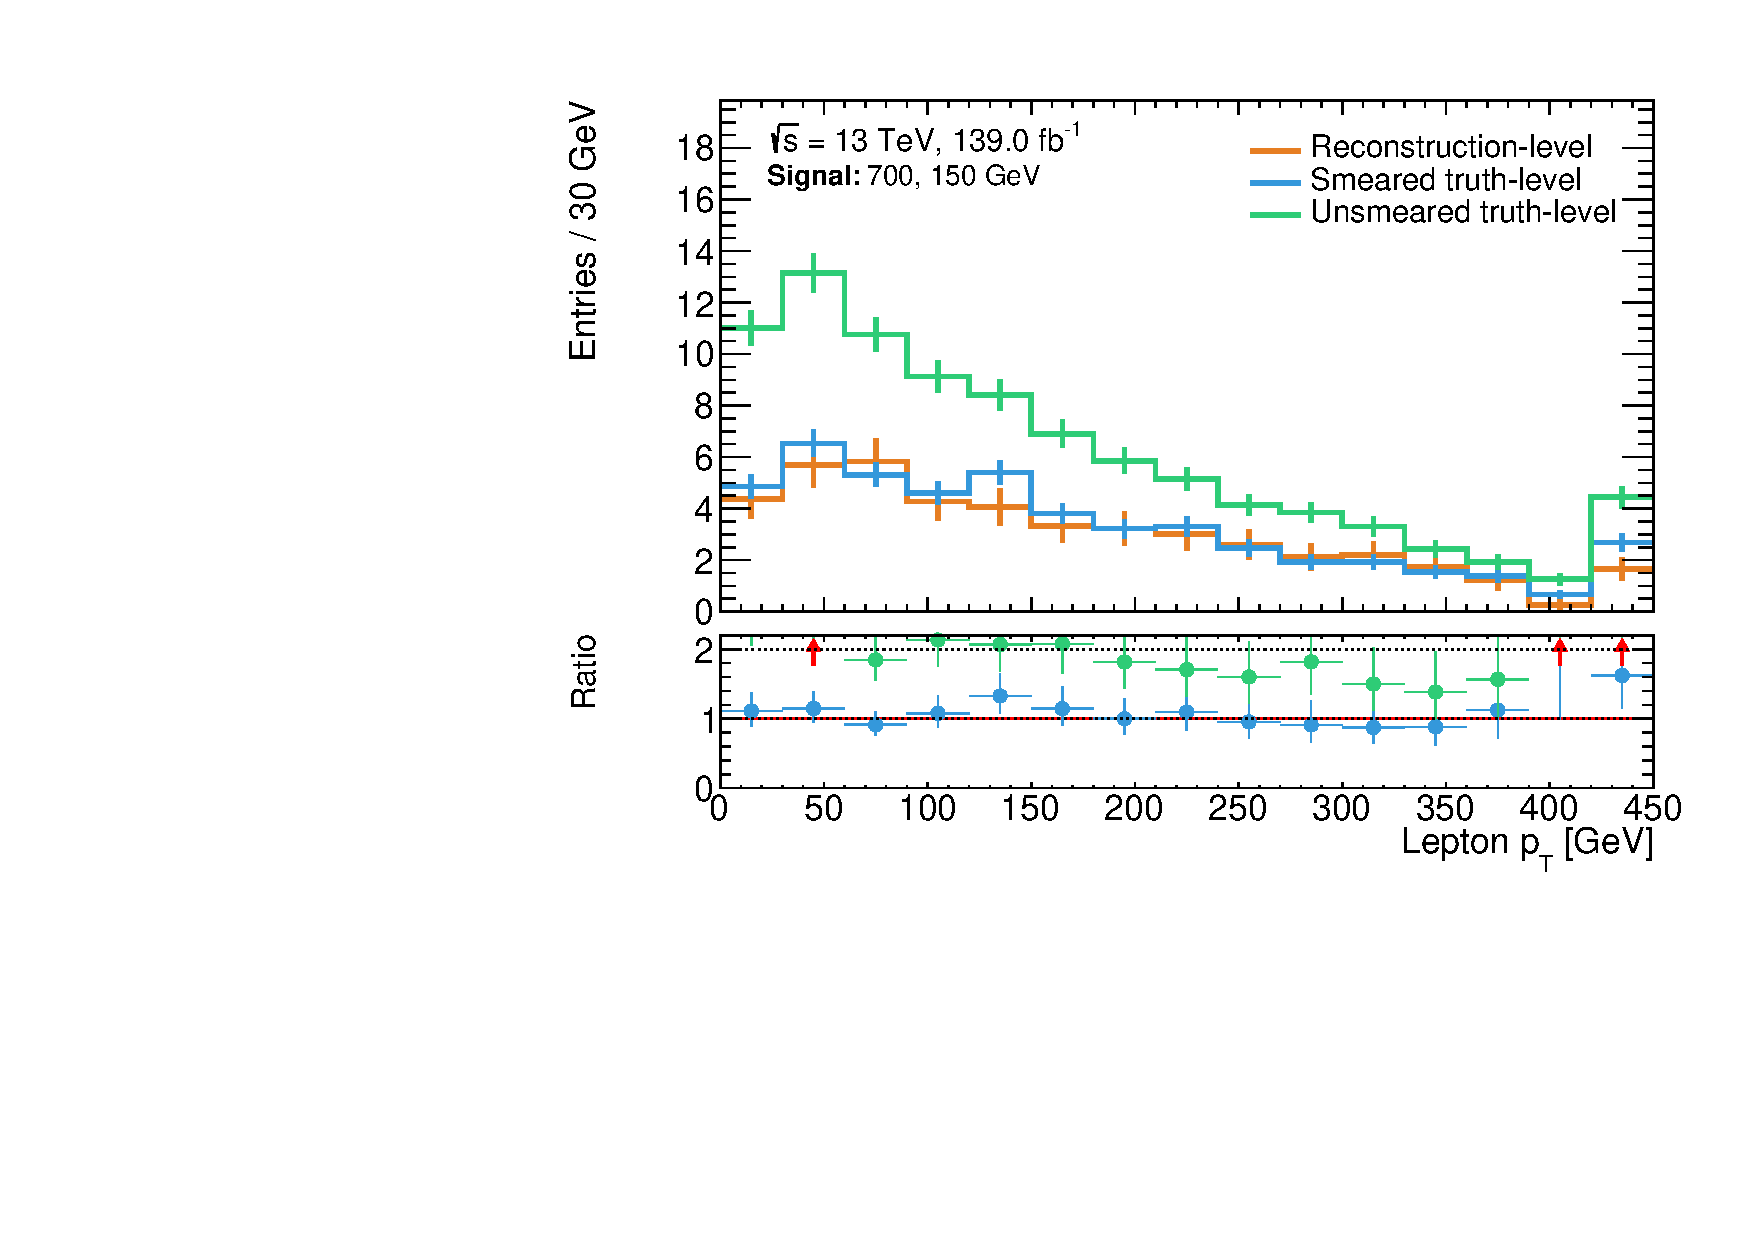
\includegraphics[width=\textwidth]{20210324/700_150/lep1Pt_C1N2_Wh_hbb_700p0_150p0_smeared.pdf}
	\end{subfigure}\hfill
	\begin{subfigure}[b]{0.45\linewidth}
		\centering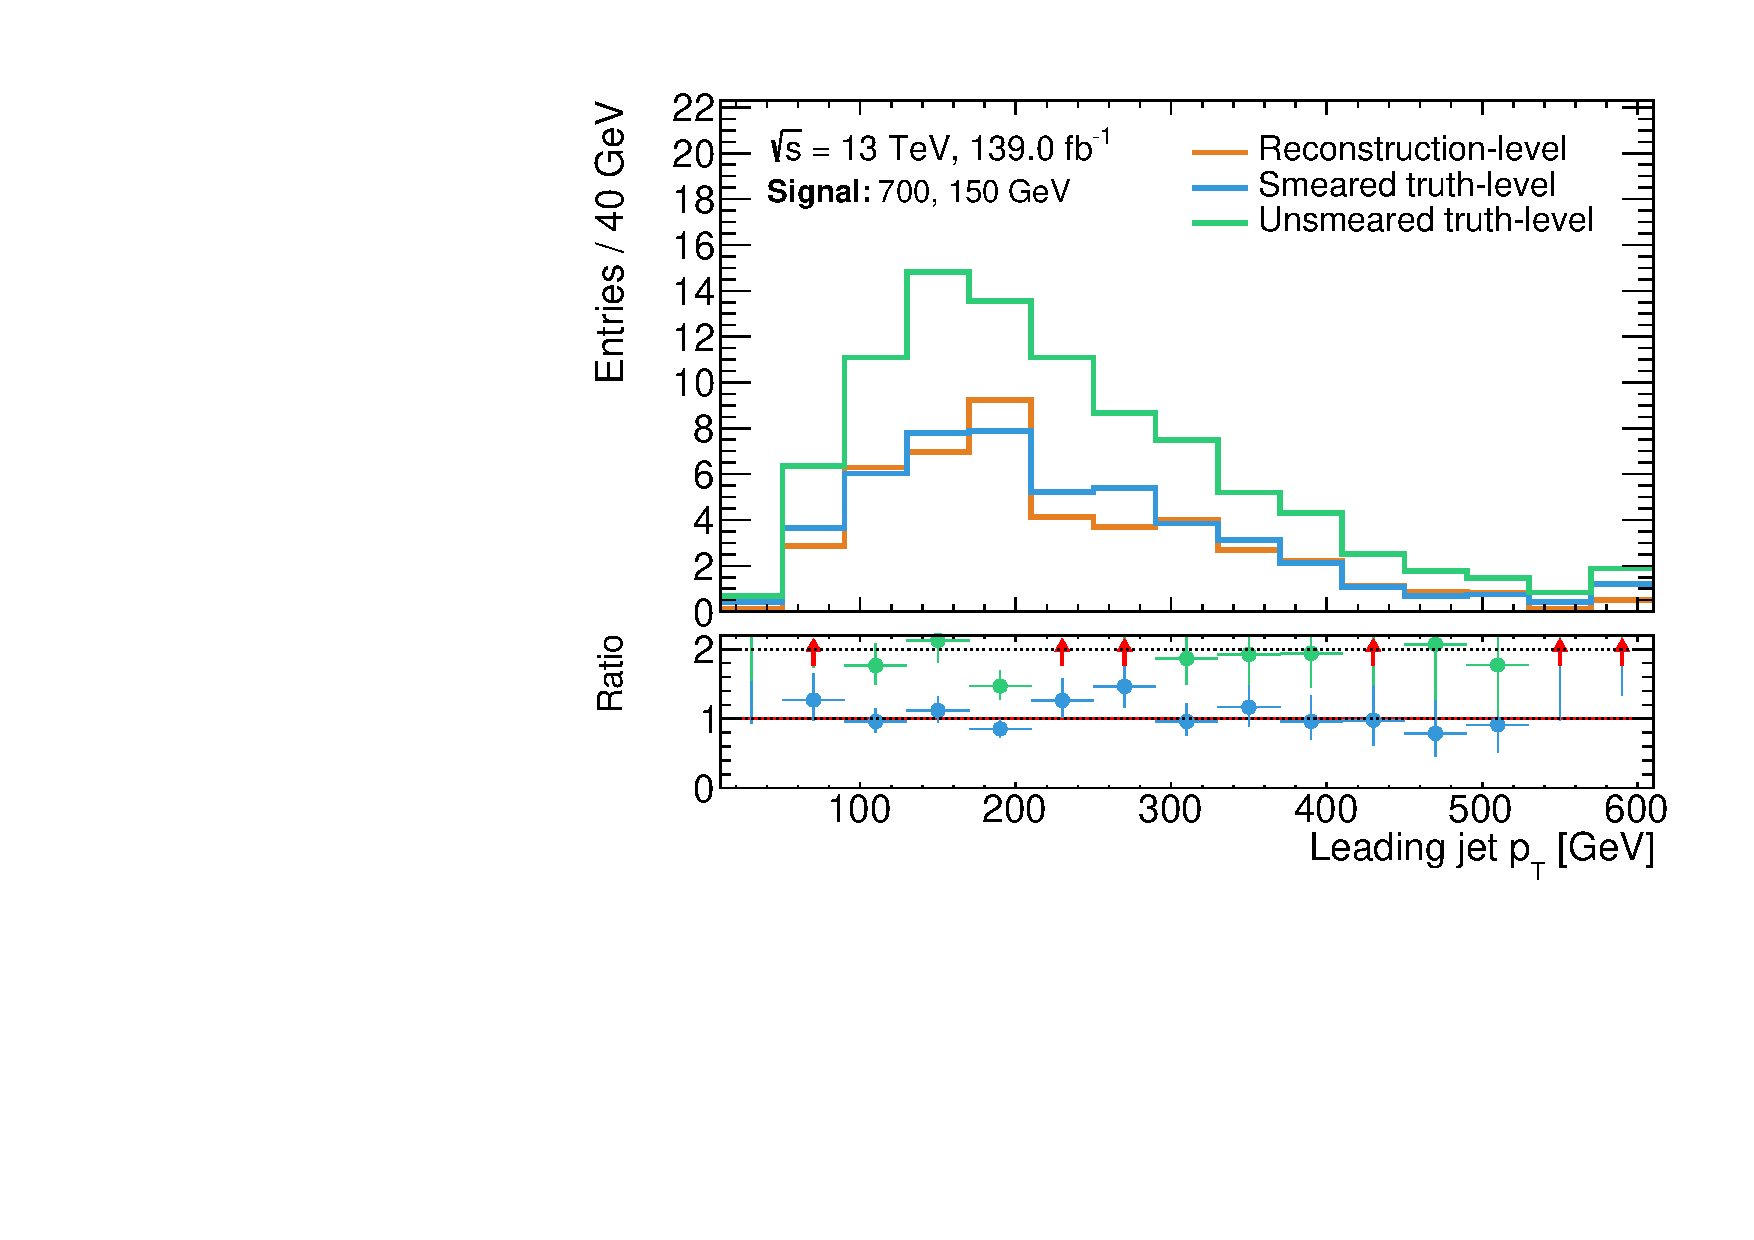
\includegraphics[width=\textwidth]{20210324/700_150/jet1Pt_C1N2_Wh_hbb_700p0_150p0_smeared.pdf}
	\end{subfigure}\hfill
	\begin{subfigure}[b]{0.45\linewidth}
		\centering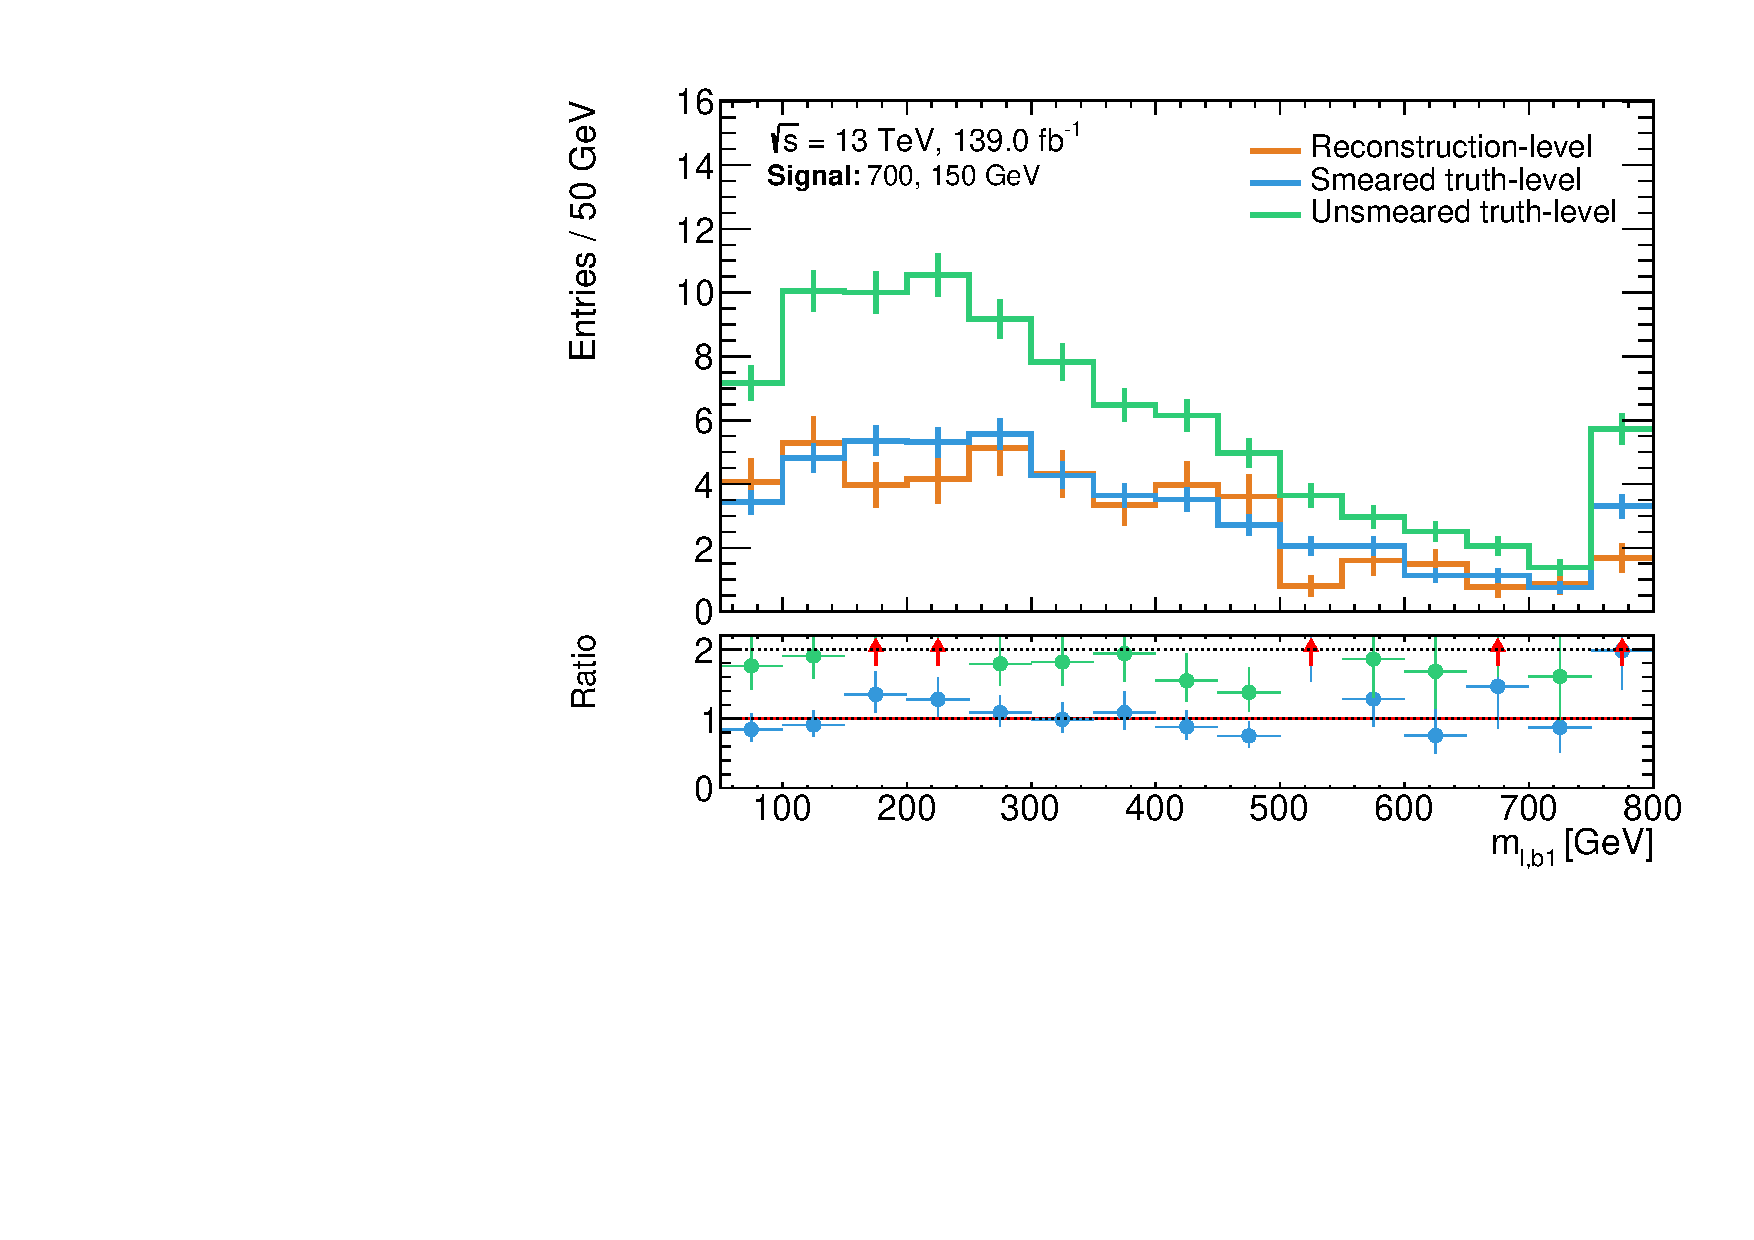
\includegraphics[width=\textwidth]{20210324/700_150/mlb1_C1N2_Wh_hbb_700p0_150p0_smeared.pdf}
	\end{subfigure}\hfill
	\begin{subfigure}[b]{0.45\linewidth}
		\centering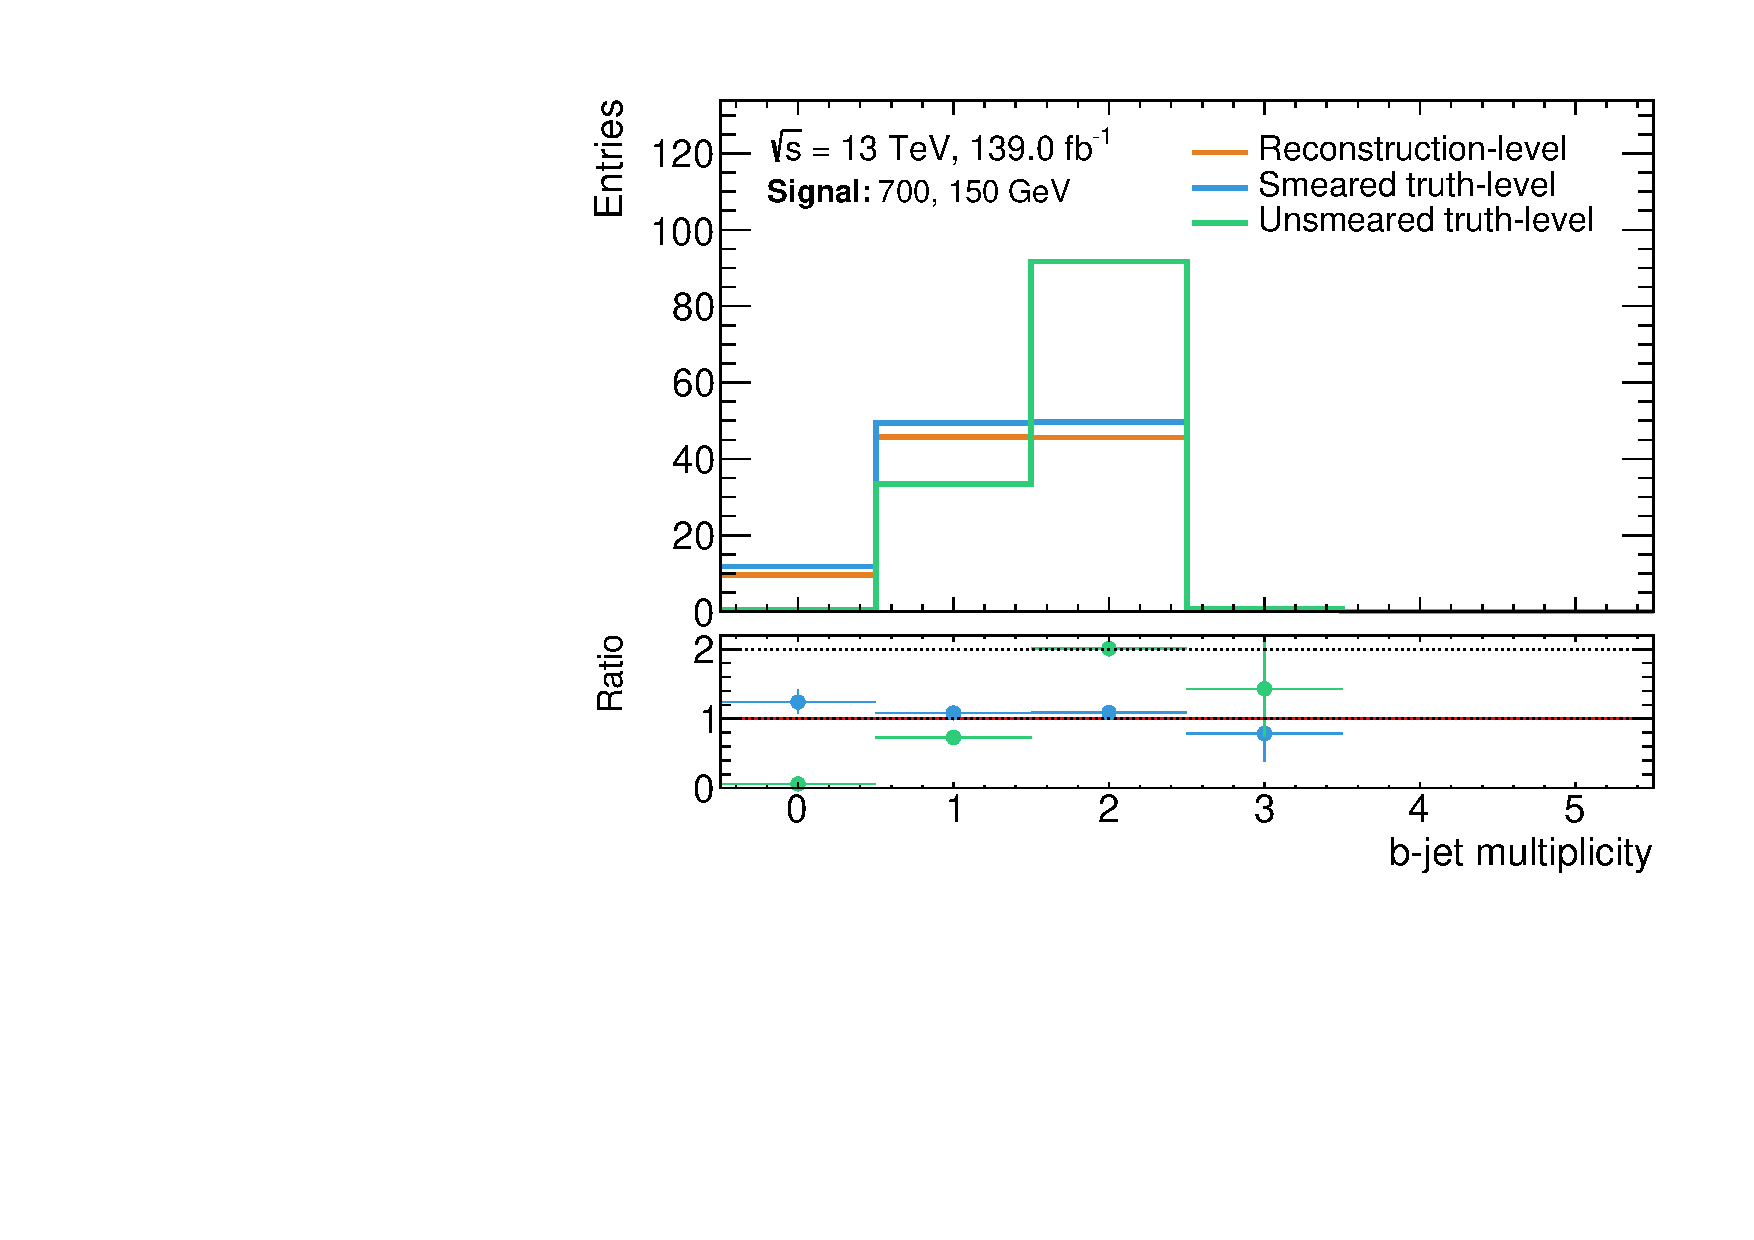
\includegraphics[width=\textwidth]{20210324/700_150/nBJet30_C1N2_Wh_hbb_700p0_150p0_smeared.pdf}
	\end{subfigure}\hfill
	\caption{Comparisons of the kinematic distributions of key observables at (smeared) truth- and reconstruction-level. The exemplary benchmark signal point with $m(\charg/\neutr), m(\lsp) = 700, \SI{150}{\GeV}$ is shown. The ratio pad shows the ratio between smeared and unsmeared truth-level distributions (blue and green) to reconstruction-level distributions (orange). Only \gls{mc} statistical uncertainty is included in the error bars. All distributions are shown in a loose preselection requiring exactly one lepton, $\met>\SI{50}{\GeV}$, $\mt > \SI{50}{\GeV}$, and 2--3 jets, two of which need to be \textit{b}-tagged. The latter requirement is dropped for the \textit{b}-jet multiplicity distribution.}
	\label{fig:smearing_preselection}
\end{figure}
 
\section{Validation of the truth-level analysis}

\subsection{Validation in loose preselection}

 The performance of the truth smearing is illustrated in a loose preselection for a single exemplary benchmark signal point in~\cref{fig:smearing_preselection}. The loose preselection applied requires exactly one lepton, $\met>\SI{50}{\GeV}$, $\mt > \SI{50}{\GeV}$, and 2--3 jets, two of which need to be \textit{b}-tagged. The reconstruction-level distributions are compared with the truth-level distributions before and after truth smearing. It can clearly be observed that the truth smearing noticeably improves the agreement between the truth- and reconstruction-level distributions. While the lepton and jet reconstruction and identification efficiencies are---due to their dependence on $\eta$, $\pt$ and individual working points---crucial for the overall agreement in shape, the inclusion of flavour-tagging efficiencies significantly improves the overall agreement in normalisation.
 
Although some minor differences remain, overall a good agreement is observed across all relevant kinematic distributions at loose preselection level. Most of the differences between smeared truth-level and reconstruction-level distributions in individual bins are well within the \gls{mc} statistical uncertainties arising from the relatively limited \gls{mc} statistics available.
 
 \subsection{Validation in signal regions}

 \begin{figure}
	\centering
	\begin{subfigure}[b]{0.49\linewidth}
		\centering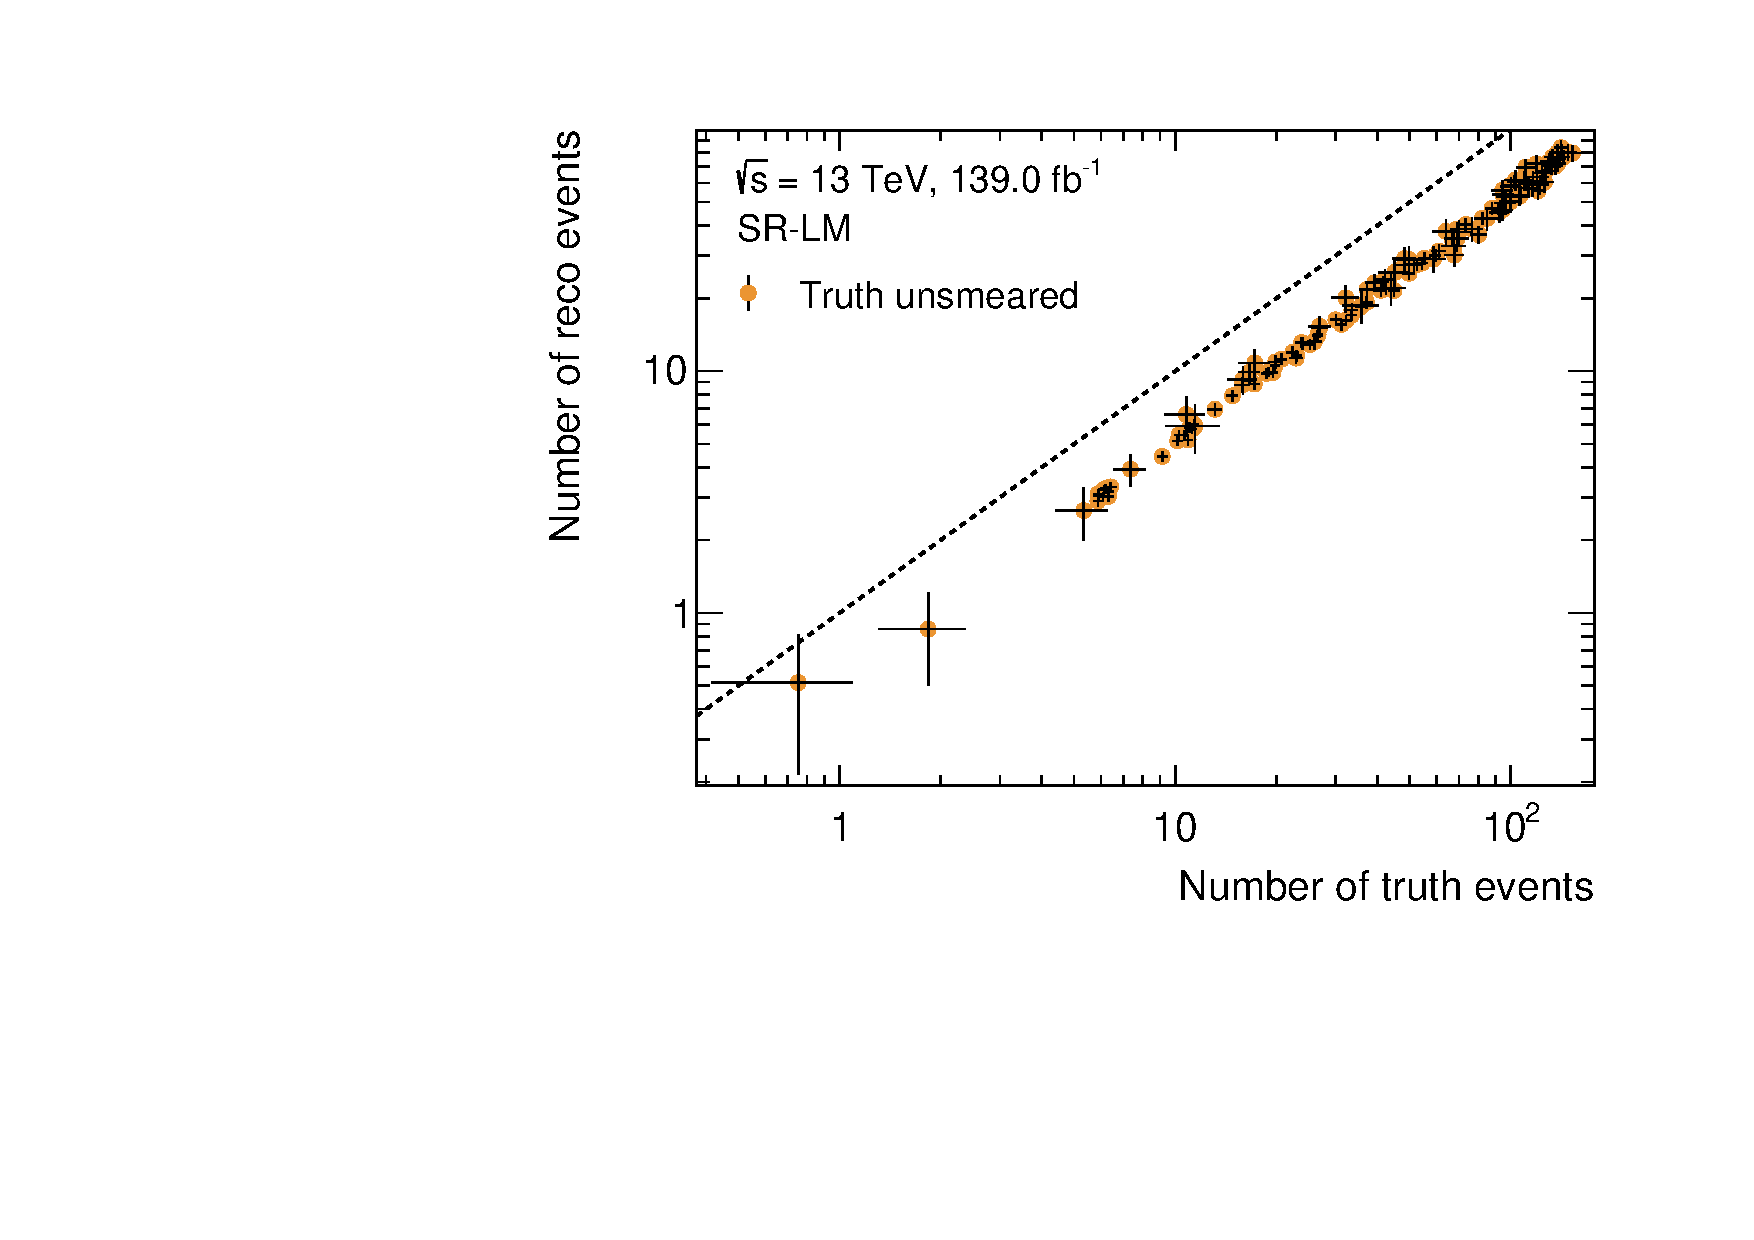
\includegraphics[width=\textwidth]{yields_SR-LM_unsmeared}
	\end{subfigure}\hfill
	\begin{subfigure}[b]{0.49\linewidth}
		\centering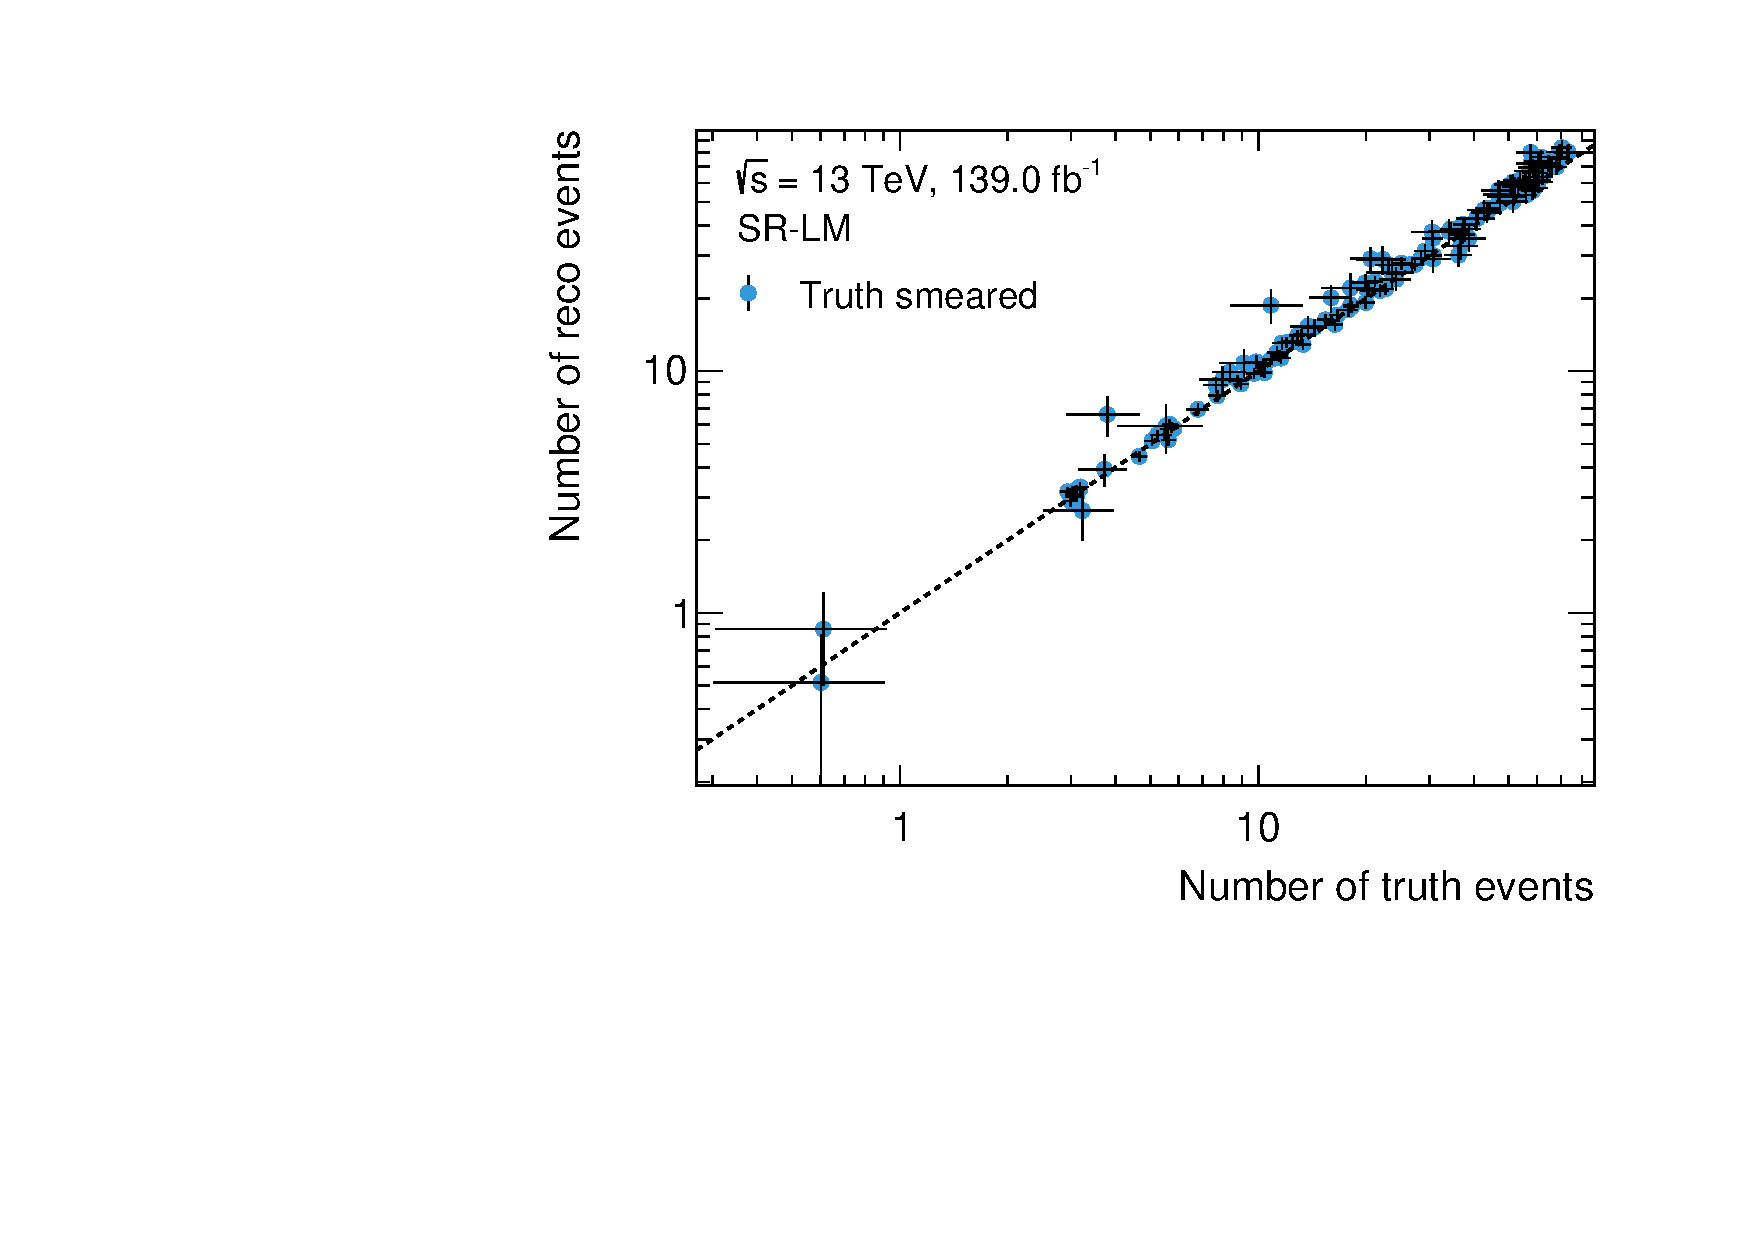
\includegraphics[width=\textwidth]{yields_SR-LM_smeared}
	\end{subfigure}\hfill
	\begin{subfigure}[b]{0.49\linewidth}
		\centering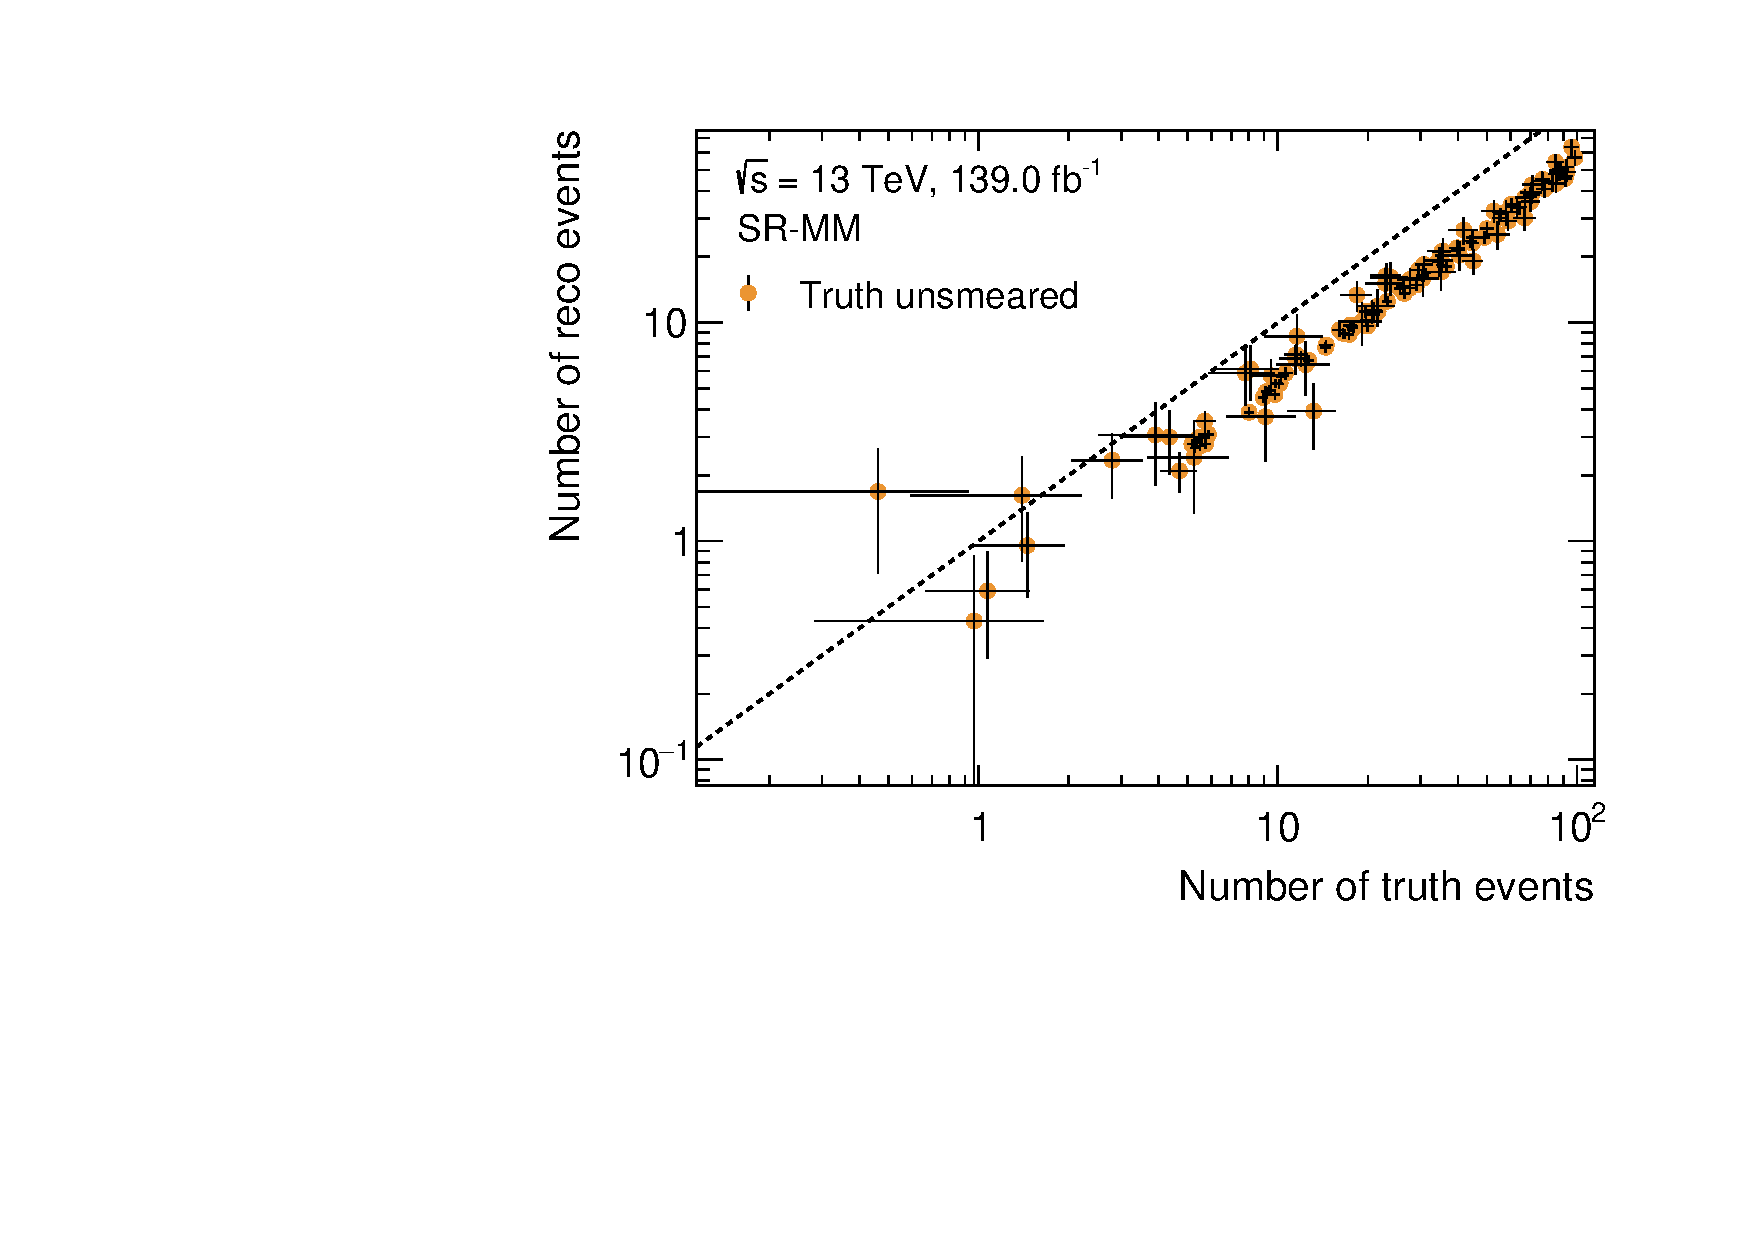
\includegraphics[width=\textwidth]{yields_SR-MM_unsmeared}
	\end{subfigure}\hfill
	\begin{subfigure}[b]{0.49\linewidth}
		\centering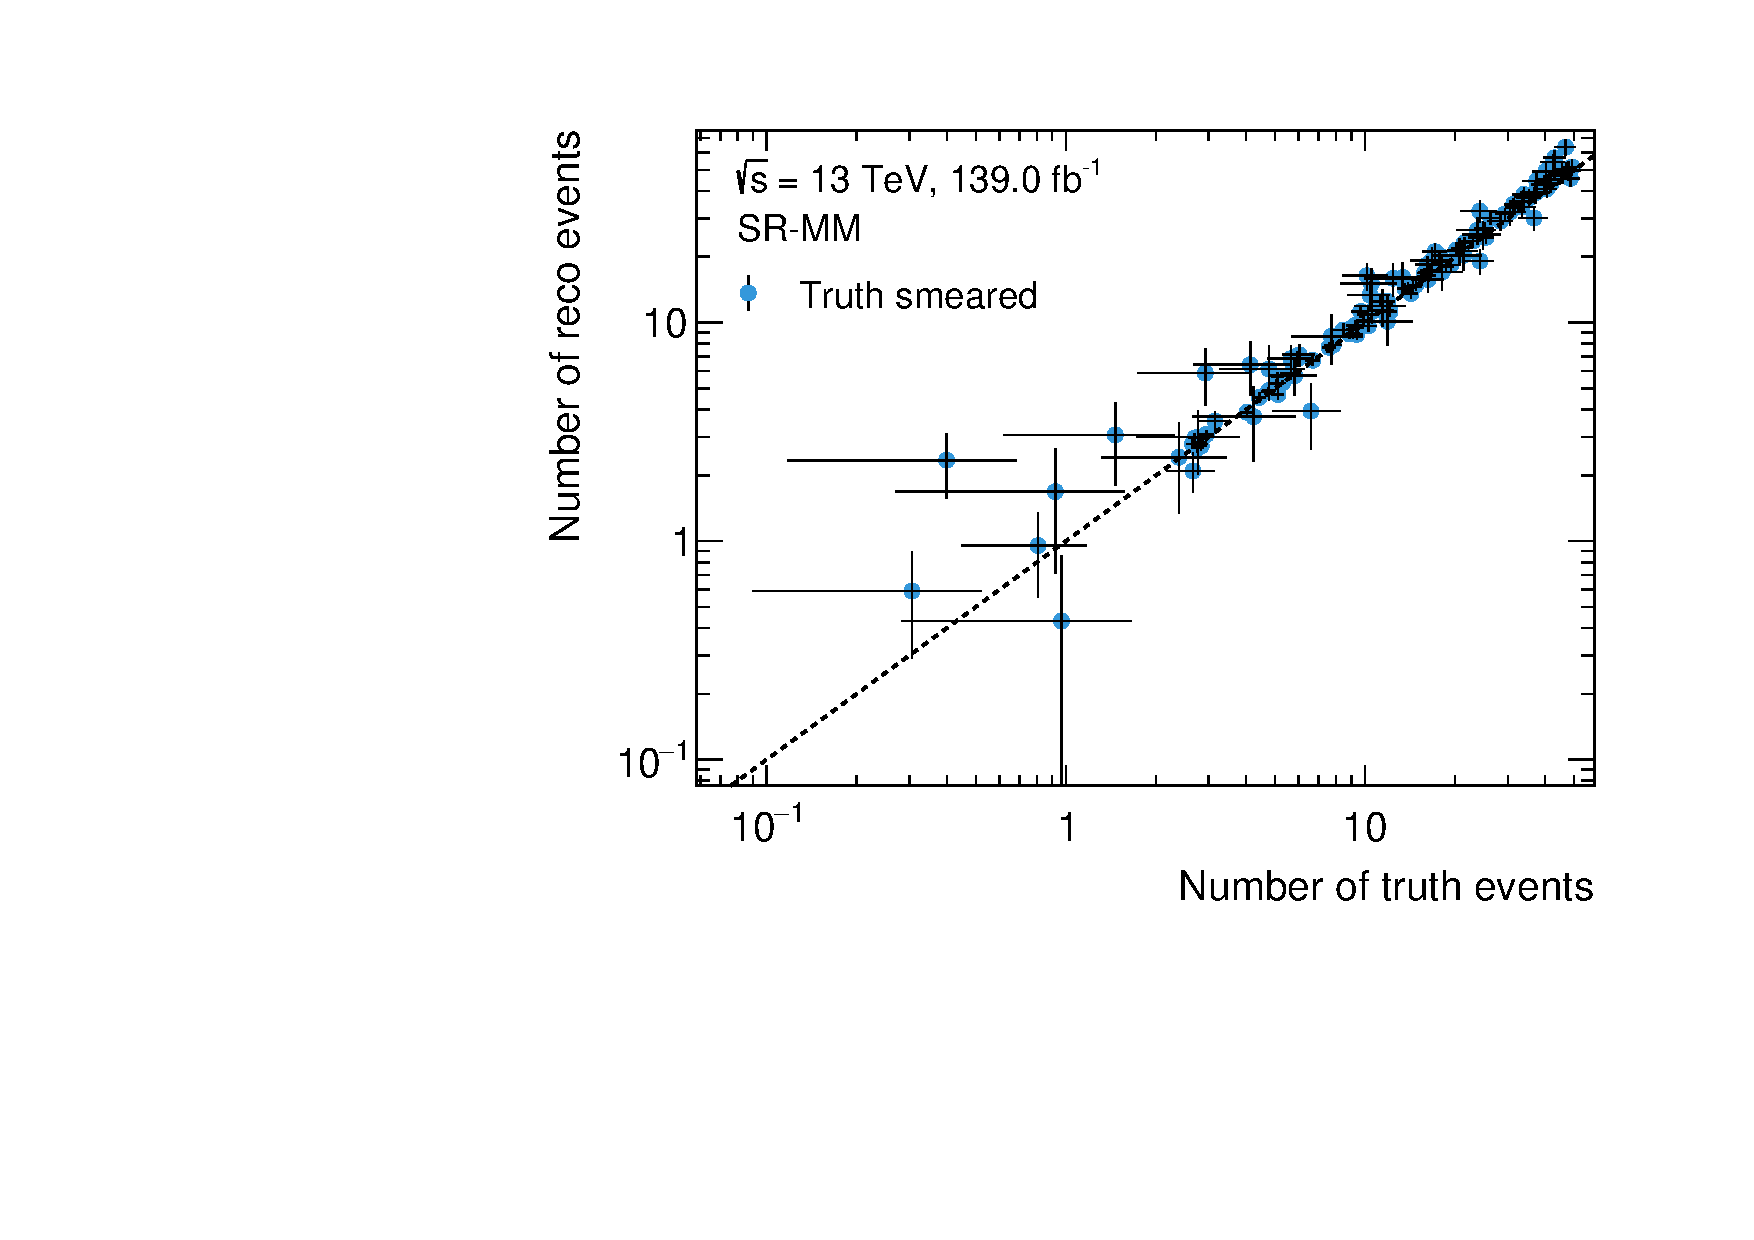
\includegraphics[width=\textwidth]{yields_SR-MM_smeared}
	\end{subfigure}\hfill
	\begin{subfigure}[b]{0.49\linewidth}
		\centering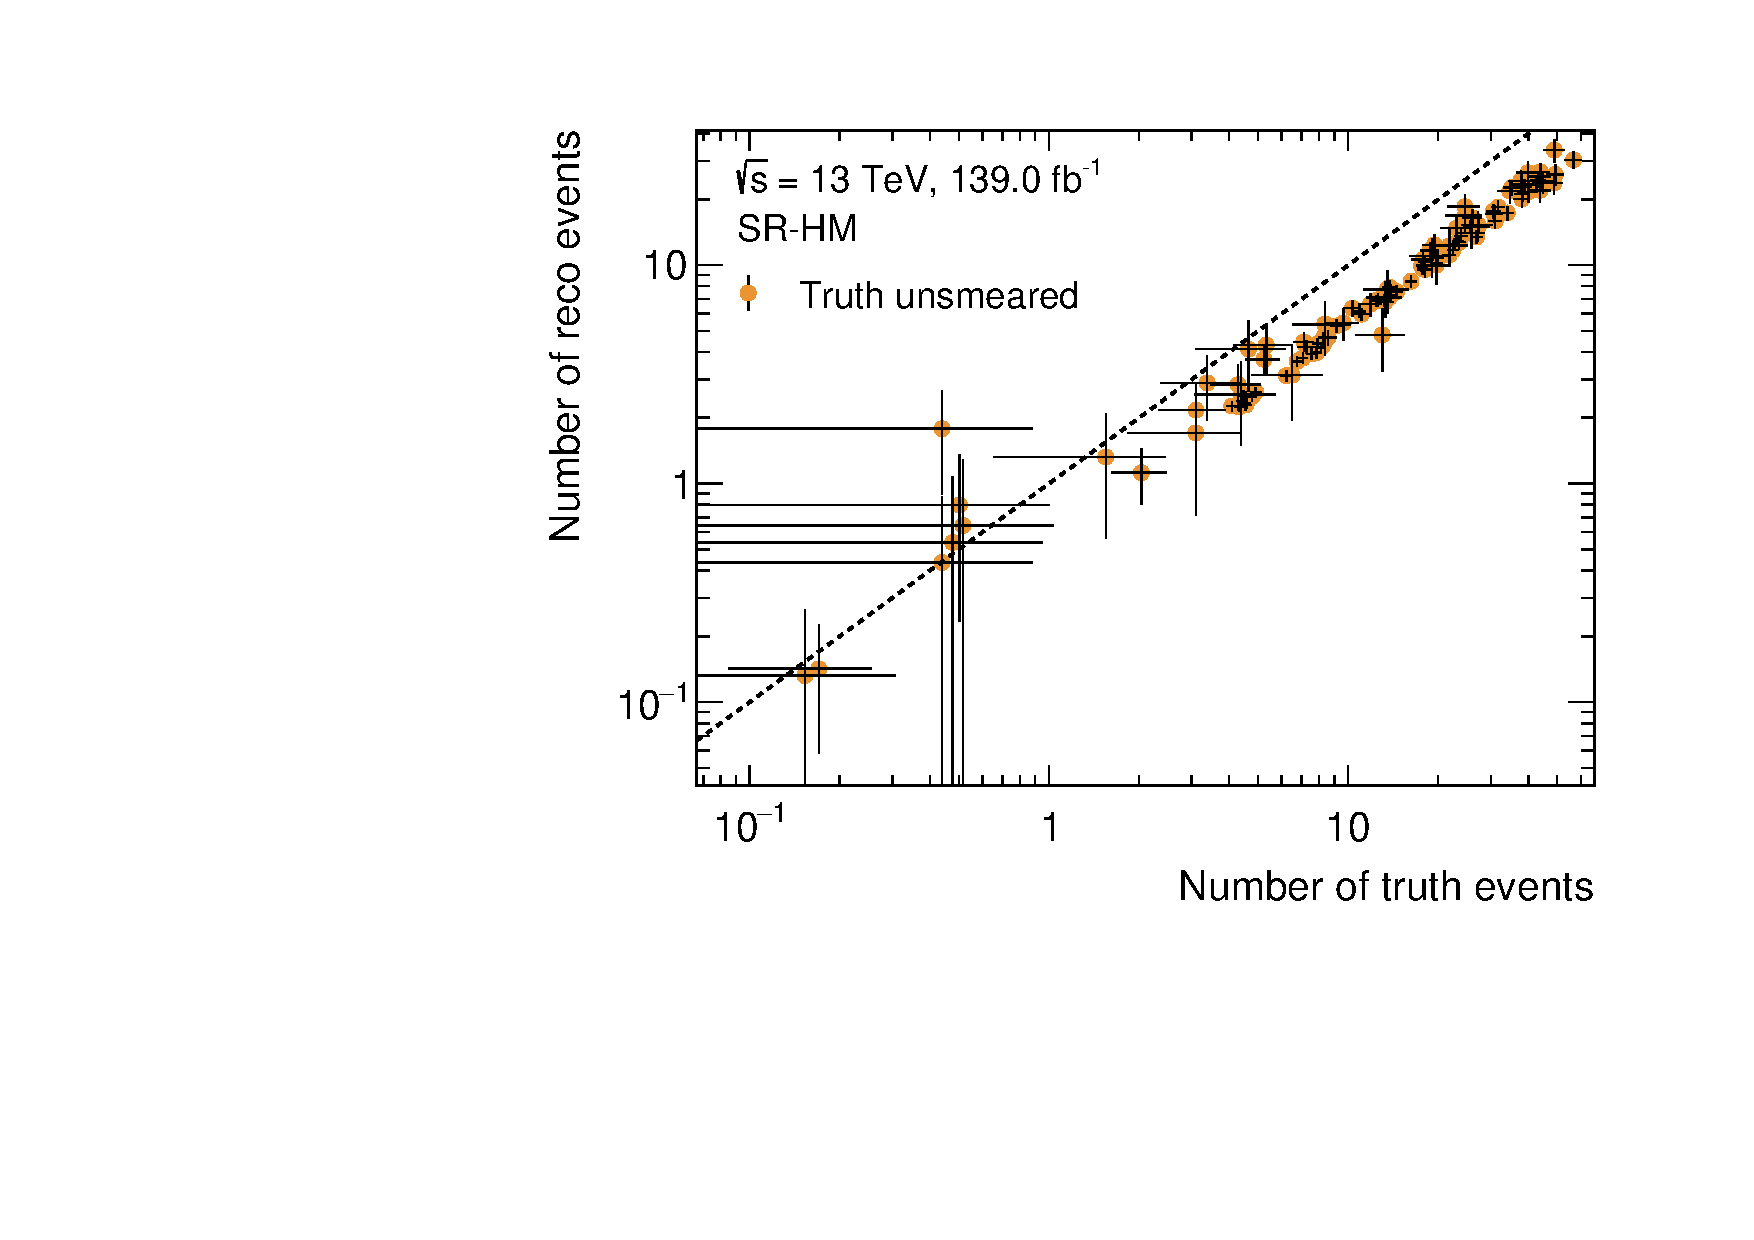
\includegraphics[width=\textwidth]{yields_SR-HM_unsmeared}
	\end{subfigure}\hfill
	\begin{subfigure}[b]{0.49\linewidth}
		\centering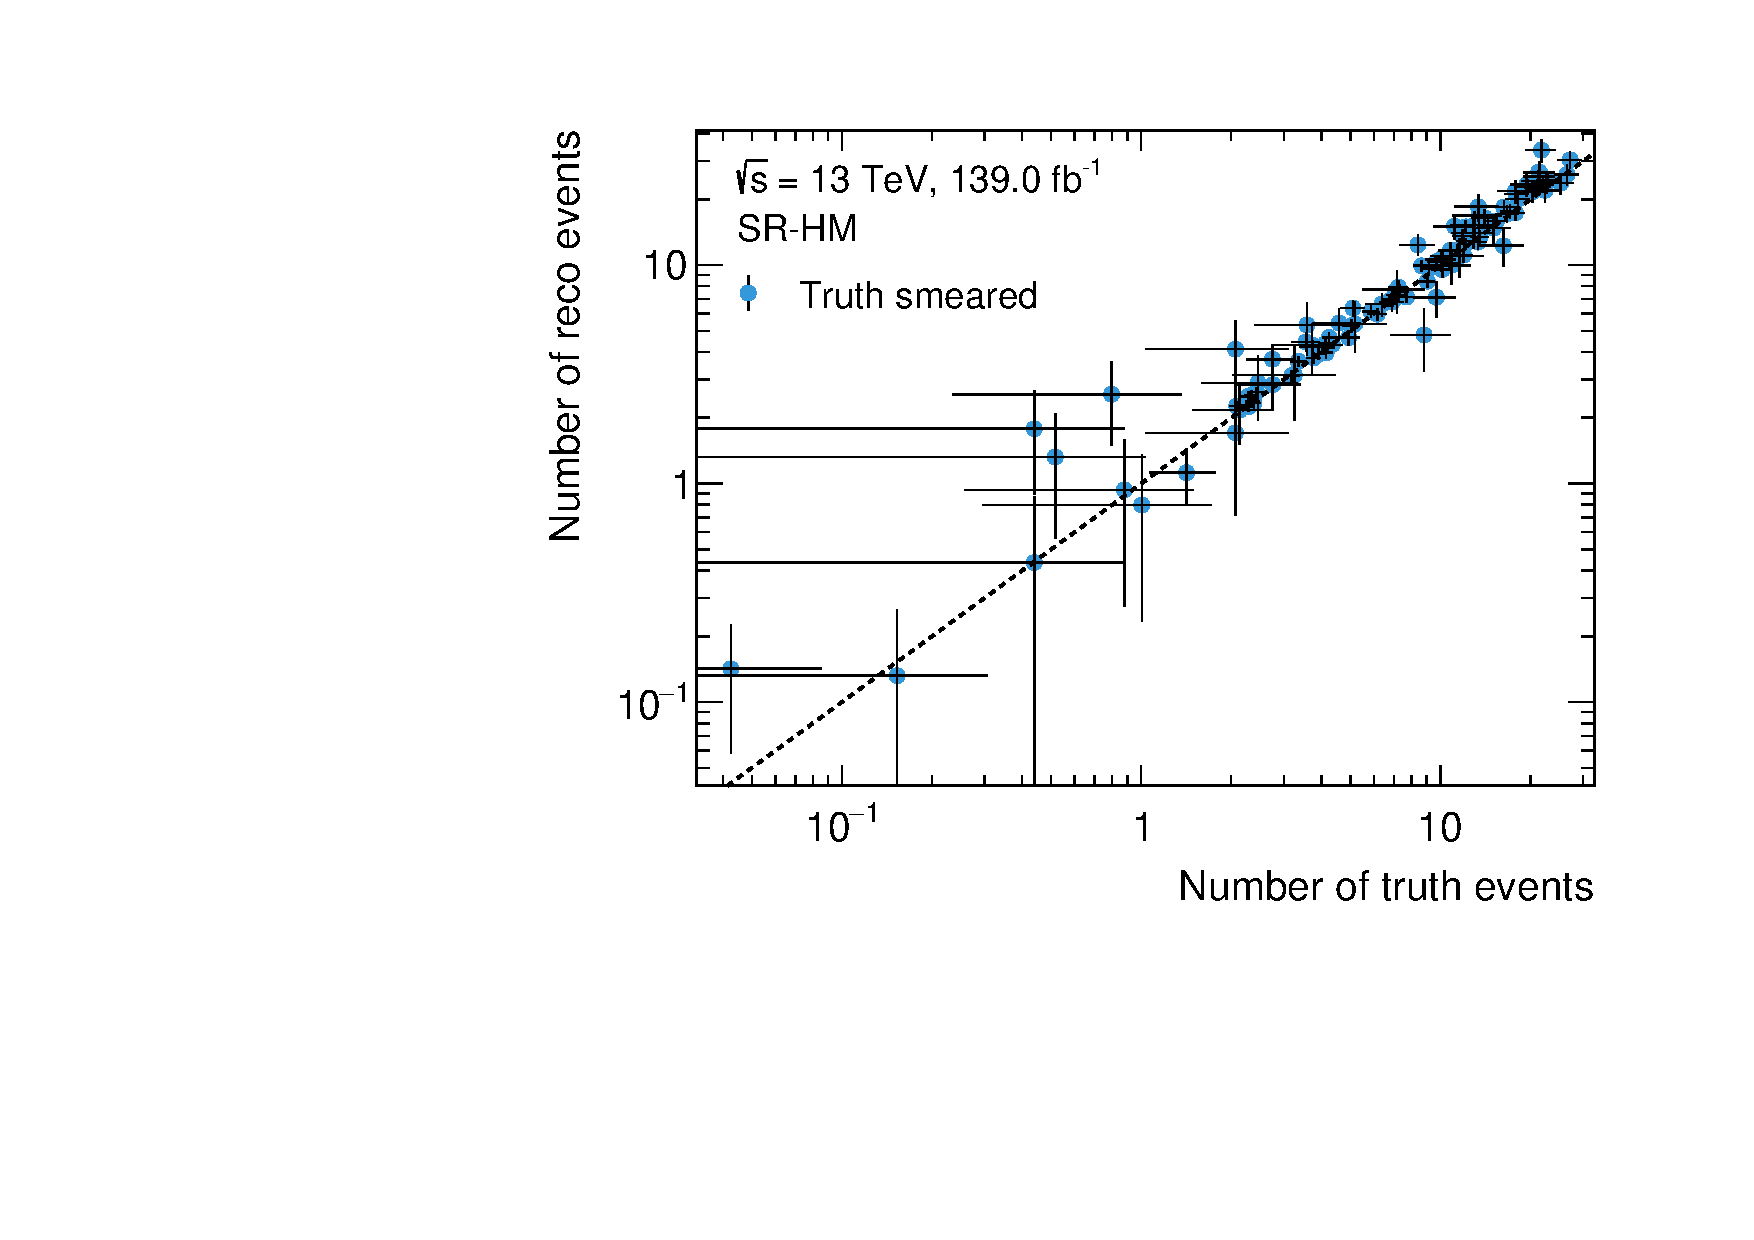
\includegraphics[width=\textwidth]{yields_SR-HM_smeared}
	\end{subfigure}
	\caption{Comparison of the event rates at truth- and reconstruction-level before (left) and after (right) truth smearing. From top to bottom, the SR-LM, SR-MM and SR-HM signal regions are shown, with cumulative (integrated) $\mct$ bins. Every single point in the scatter plots represents a single signal model considered in the original 1-lepton analysis. Uncertainties include \gls{mc} statistical uncertainties.}
	\label{fig:smearing_signal_regions}
\end{figure}
 
 As the expected signal rates in the signal regions are ultimately what is entering the (simplified) likelihood, it is important that the good agreement observed at preselection is still present in the kinematically tighter selections of the signal regions. Additionally, it is worth investigating the agreement across all signal models considered in the original analysis, as opposed to only validating specific benchmark points. A comparison of the reconstruction-level and truth-level event rates before and after smearing in the signal regions SR-LM, SR-MM and SR-HM is shown in~\cref{fig:smearing_signal_regions} for all signal models considered in the 1-lepton analysis. For the sake of conciseness, only the cumulative $\mct$ bins are shown in each \gls{sr} in~\cref{fig:smearing_signal_regions}. The agreement in the individual $\mct$ bins in each SR-LM, SR-MM and SR-HM is provided in~\cref{fig:smearing_signal_regions_1,fig:smearing_signal_regions_2,fig:smearing_signal_regions_3}.
 
The truth smearing drastically improves the agreement in event rate estimates at truth- and reconstruction-level across all \gls{sr} bins considered. While the event rates are generally overestimated at truth-level before smearing, compared to reconstruction-level, both tend to agree well within statistical uncertainties after smearing. 
 
\subsection{Validation using likelihood}


 \begin{figure}
	\centering
	\begin{subfigure}[b]{0.49\linewidth}
		\centering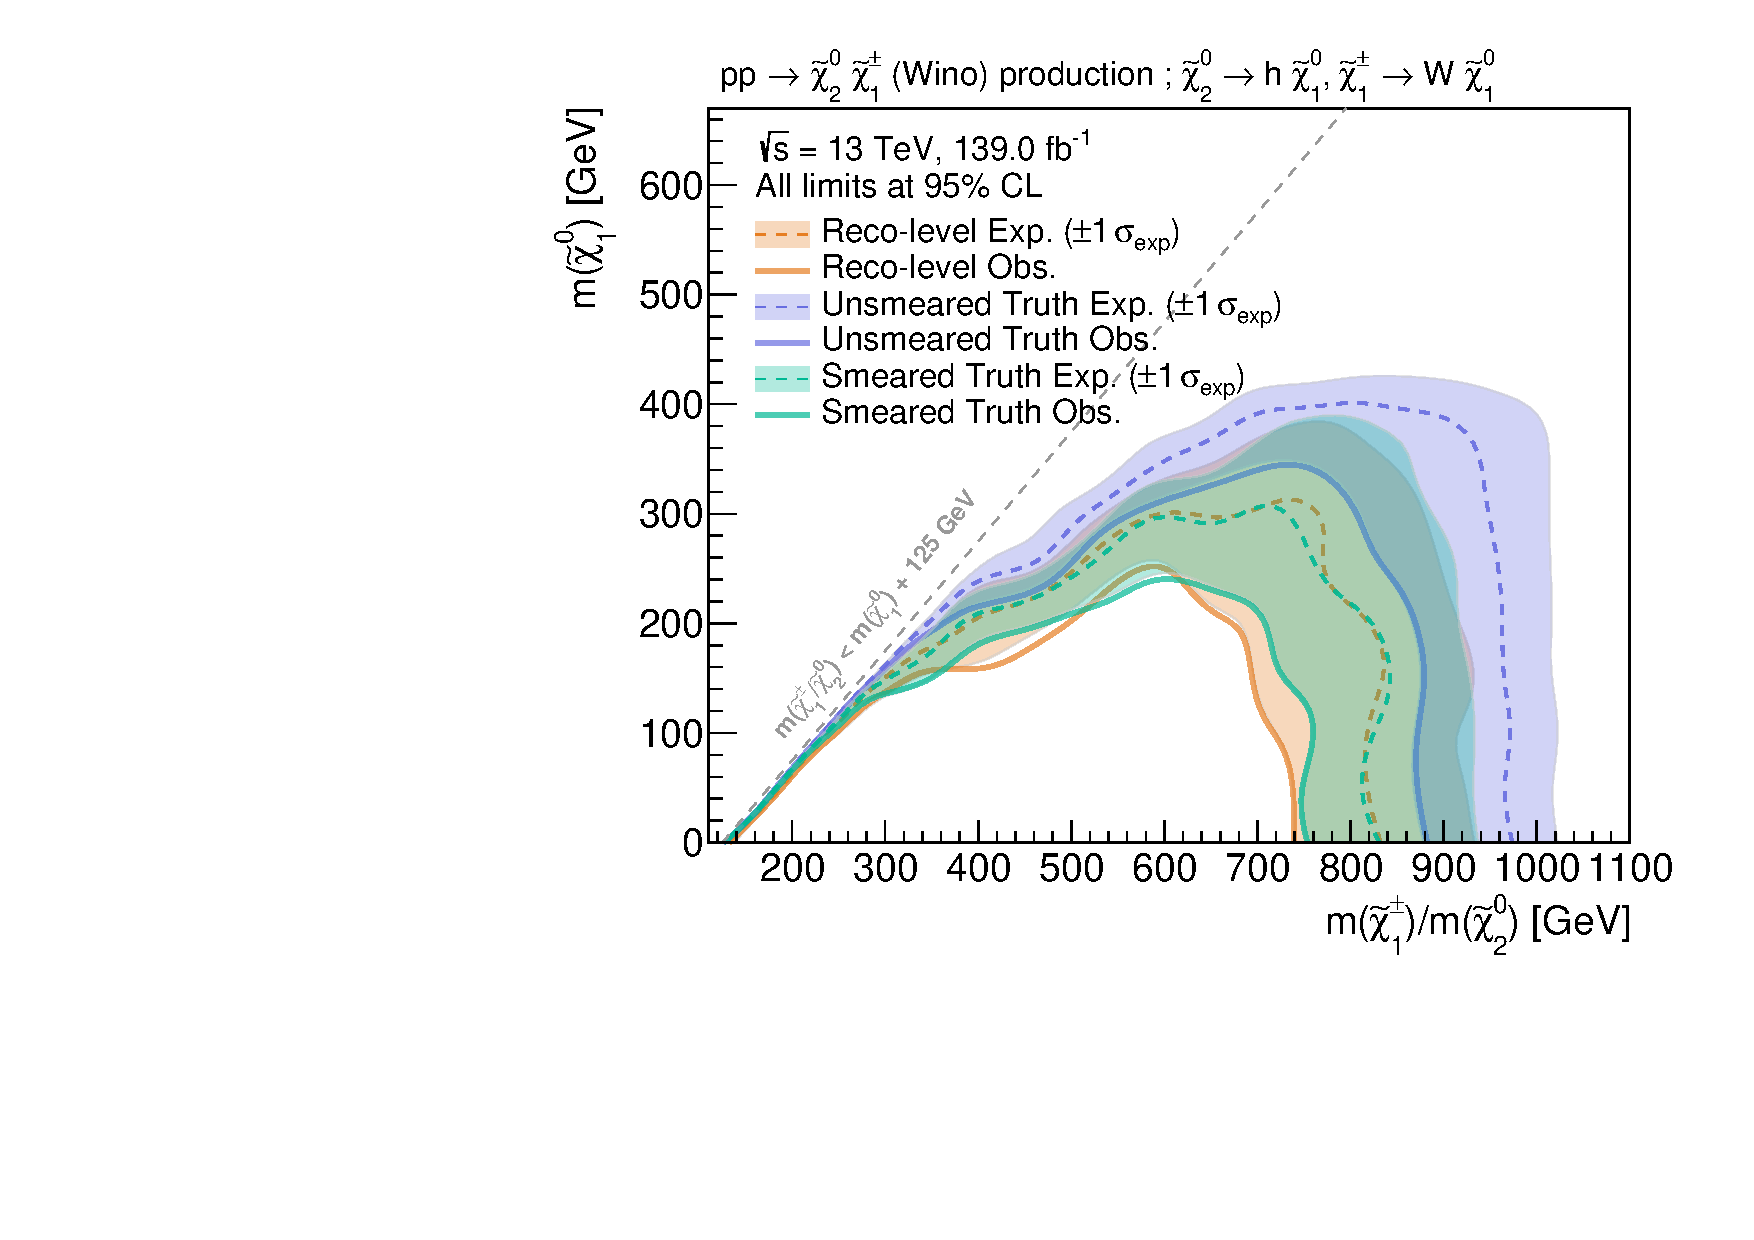
\includegraphics[width=\textwidth]{exclusion_1Lbb_truthInput_compareReco_BkgOnly_noLabel}
		\caption{\label{fig:full_truth_result}}
	\end{subfigure}\hfill
	\begin{subfigure}[b]{0.49\linewidth}
		\centering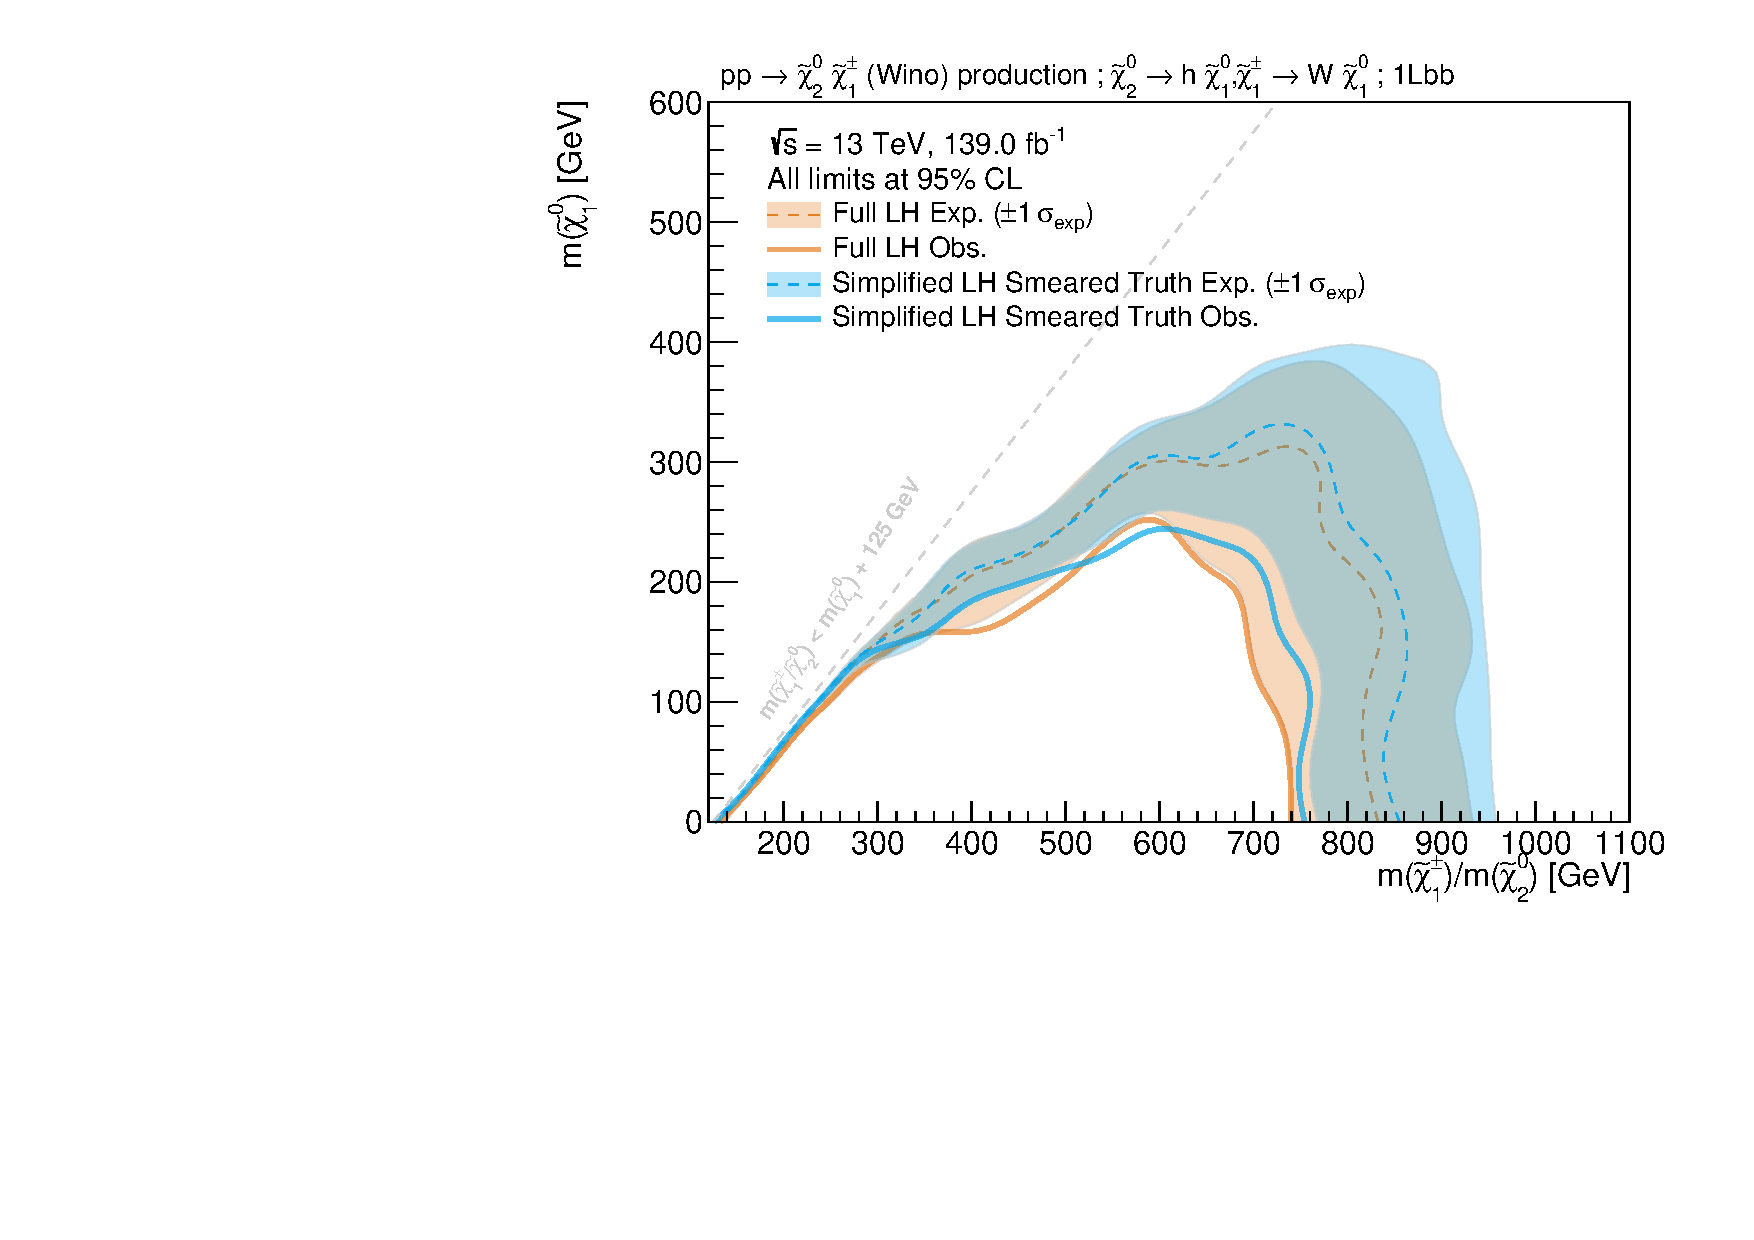
\includegraphics[width=\textwidth]{exclusion_1Lbb_truthInput_BkgSignal_700_200_noLabel}
		\caption{\label{fig:simplified_truth_result}}
	\end{subfigure}\hfill
	\caption{Expected and observed exclusion contours obtained with the full and simplified likelihoods. Fig.~\subref{fig:full_truth_result} compares the full likelihood contours obtained with the reconstruction-level inputs (orange) to results obtained with truth inputs before (purple) and after (green) smearing. Fig.~\subref{fig:simplified_truth_result} compares the full likelihood reconstruction-level contours (orange) with those obtained using the simplified likelihood and smeared truth-level inputs (blue). Uncertainties include all statistical and systematic uncertainties on the background and signal for the reconstruction-level contours, but only statistical and systematic uncertainties on the background for truth-level signal inputs.}
	\label{fig:smearing_signal_regions}
\end{figure}

Using the nominal expected event rates at smeared truth-level for every signal model in the original signal grid considered in the 1-lepton analysis, expected and observed CL$_s$ values can be computed and exclusion contours can be derived. \Cref{fig:full_truth_result} compares the expected and observed exclusion contours obtained using the full likelihood and reconstruction-level signal inputs with those obtained using the full likelihood and truth-level signal inputs before and after truth smearing. While all theory and systematic uncertainties on the signal are included in the reconstruction-level contours, no signal uncertainties are considered when obtaining both the smeared and unsmeared truth-level contours. As expected from the previous validation steps in the signal regions, the sensitivity using unsmeared truth-level signal inputs is significantly overestimated compared to the published analysis exclusion limit using reconstruction-level inputs. The smeared truth-level inputs, however, yield exclusion contours with an acceptable match compared to the reconstruction-level results.

With the truth smearing validated at multiple selection levels of the analysis, the full two-fold approximation of signal pipeline and statistical inference can be constructed. \Cref{fig:simplified_truth_result} compares the exclusion contours of the original analysis results with those obtained using smeared truth-level signal inputs as well as the simplified likelihood. Even with the approximations made, overall a good agreement is found and the original analysis results can be reproduced to a relatively high degree of precision.

In summary, this validation process shows that the signal pipeline in~\cref{fig:pipeline_analysis} can be efficiently approximated using truth-level analysis and a simplified treatment of the statistical model, allowing a considerably faster evaluation of \gls{bsm} models while still offering reliable results. In large-scale reinterpretations, this approach thus enables an efficient classification of models into safely excluded and non-excluded models as well as models where exclusion is in doubt and where the full analysis pipeline using \textsc{Recast} is needed.


